\documentclass[letterpaper,12pt]{report}
\usepackage{thesis}
\usepackage{amsmath}
\usepackage{amsfonts}
\usepackage{amssymb}
\usepackage{hyperref}
\usepackage{xcolor}

%% Comments
\newif\ifcomments\commentstrue

\ifcomments
\newcommand{\authornote}[3]{\textcolor{#1}{[#3 ---#2]}}
\newcommand{\todo}[1]{\textcolor{red}{[TODO: #1]}}
\else
\newcommand{\authornote}[3]{}
\newcommand{\todo}[1]{}
\fi

\newcommand{\wss}[1]{\authornote{blue}{SS}{#1}} %Spencer Smith
\newcommand{\jc}[1]{\authornote{red}{JC}{#1}} %Jacques Carette
\newcommand{\oo}[1]{\authornote{magenta}{OO}{#1}} %Olu Owojaiye
\newcommand{\pmi}[1]{\authornote{green}{PM}{#1}} %Peter Michalski
\newcommand{\ad}[1]{\authornote{brown}{AD}{#1}} %Ao Dong

%\textwidth 5in

\newcommand{\shorttitle}{State of Practice for Medical Imaging Software}
\newcommand{\fulltitle}{Assessing the Current State of the Practice for Medical Imaging Software}
\newcommand{\authorname}{Ao Dong}

\begin{document}

\pagenumbering{roman}

\thesisshorttitle {\MakeUppercase{\shorttitle}}

\thesistitle
	{\MakeUppercase{\fulltitle}}
	{\MakeUppercase{\authorname}.}
	{Master of Engineering in Computing and Software}
	{\copyright \ Copyright by Ao Dong, August 2021}

\descriptivenote{a descriptive note}

\addcontentsline{toc}{chapter}{Abstract}
\begin{center}
\textbf{\large Abstract}
\end{center}

\begingroup
\setstretch{1.25}
We present a general method to assess the state of the practice for Scientific Computing (SC) software and apply the method to the Medical Imaging (MI) software. This method guided us to select 29 MI software projects from 48 candidates, assess 10 software qualities (\textit{Installability}, \textit{Correctness \& Verifiability}, \textit{Reliability}, \textit{Robustness}, \textit{Usability}, \textit{Maintainability}, \textit{Reusability}, \textit{Understandability}, \textit{Visibility/Transparency}, and \textit{Reproducibility}) by answering 103 questions for each software, and interview eight of the 29 development teams. The results helped us with revealing the current status of MI software development. Based on the quantitative data for the first nine qualities, we ranked the MI software with the Analytic Hierarchy Process (AHP). The top three software products were \textit{3D Slicer}, \textit{ImageJ}, and \textit{OHIF Viewer}, which received high scores for most qualities. \textit{3D Slicer} was among the top two for all nine qualities except \textit{robustness}. By interviewing the developers, we identified three major types of pain points during their development process: i) the lack of resources; ii) the difficulty to balance between four factors: \textit{compatibility}, \textit{maintainability}, \textit{performance}, and \textit{security};
iii) the lack of access to real-world datasets for testing. We collected proven and potential solutions for these problems. The interviews also helped us to understand the status of documentation, project management, and five qualities (\textit{correctness}, \textit{maintainability}, \textit{understandability}, \textit{usability}, and \textit{reproducibility}) in the projects. We summarized the threats and strategies to these qualities. For future SC software development, we proposed recommendations on improving software qualities, dealing with limited resources, choosing a tech stack, and enriching the testing datasets. The recommendations include adopting test-driven development, using continuous integration and continuous delivery (CI/CD), using git and GitHub, maintaining good documents, supporting third-party plugins or extensions, considering web application solutions, and establishing community collaboration in a SC domain.  \newline

\noindent\textbf{Keywords:} Medical Imaging, Scientific Computing, software engineering, software quality, Analytic Hierarchy Process, developer interview
\endgroup

\addcontentsline{toc}{chapter}{Acknowledgments}
\begin{center}
\textbf{\textup{\Large Acknowledgments}}
\end{center}

acknowledgements here
\tableofcontents
\label{lastoffront}


\pagestyle{fancy}
%\fancyhf{}
\renewcommand{\headrulewidth}{0in}
\chead{MEng Thesis - \authorname - McMaster - Computing and Software}\ \   
\lhead{}
\rhead{}

% \pagestyle{headings}
\markboth{MASc Thesis - \authorname - McMaster - Computing and Software}{}

\pagenumbering{arabic}

\chapter{Introduction}
\label{ch_intro}
We define Scientific Computing (SC) as ``the use of computer tools to analyze or simulate mathematical models of real world systems of engineering or scientific importance so that we can better understand and predict the system’s behaviour" \cite{Smith2006}. Many researchers consider SC as the third pillar of science and engineering, along with theory and experiment \cite{Landau2005}. Almost all areas in science and engineering use computers for modeling \cite{Golub2014}, and software plays an essential role in modern scientific research \cite{Hannay2009} \cite{Wilson2014}.  Software development in SC depends on three fields of knowledge: engineering or scientific domain knowledge, mathematical algorithm knowledge, and computational algorithm knowledge \cite{Landau2005} \cite{Mehta2015}. Thus, most SC software developers are scientists in SC domains \cite{Wilson2014}. However, they do not always use the modern software development techniques, tools, and methods \cite{Wilson2014}. Therefore, we developed a methodology for assessing the state of the practice for SC software. We apply this process to Medical Imaging (MI) software that belongs to a specific domain of SC.

This report analyzes the state of the practice for MI software. MI is the clinical tool to image the interior of a body, providing information for diagnostic, analytic, and medical applications \cite{FDA2021} \cite{enwiki:1034887445}. MI is an essential part of collecting accurate information during clinical diagnosis \cite{Zhang2008}. MI software aims to visualize and process medical images and produce clinically meaningful information \cite{enwiki:1034877594}.

We aim to study the current status of SC software development in the MI domain; understand the current merits, drawbacks, and pain points during the development process, as well as the software qualities in the domain; provide guidelines and recommendations for future development.

Section \ref{sec_motivation} presents our motivation to start the research set the above goals, Section \ref{sec_research_questions} lists our research questions, and Section \ref{sec_scope} presents the scope of MI software in our research.

\section{Motivation}
\label{sec_motivation}
Most scientists think developing and using SC software plays a significant role in their research \cite{Hannay2009}. They spend a substantial proportion of their working hours on SC software development \cite{Hannay2009} \cite{Prabhu2011}, and this proportion of time has increased over the years \cite{Hannay2009}. 

Developing SC software requires solid knowledge in specific domains \cite{Wilson2014}. Many developers learn software engineering skills by themselves or from their peers, instead of from proper training \cite{Hannay2009}. Hannay et al. \cite{Hannay2009} observe that many scientists showed ignorance and indifference to standard software engineering concepts. According to a survey by Prabhu et al. \cite{Prabhu2011}, more than half of the 114 subjects did not use any proper debugger for their software.

Due to its nature, SC software born from one project can be part of many other projects in the future, with the potential to disproportionately causing damages to scientific research \cite{Wilson2014}. 

As a result, the development process and quality of SC software concern us. We want to understand their status in SC domains and improve them. In addition, we want to understand whether problems like these mentioned above occur in all SC domains, or whether the state of the practice varies between domains. We build and refine our methodology, based on our previous work in scientific domains such as oceanography \cite{Smith2015}, mesh generation \cite{smith2016state}, geographic information systems \cite{smith2018state}, psychology \cite{smith2018statistical} and seismology \cite{Smith2018Seismology}. 

\section{Research Questions}
\label{sec_research_questions}
To achieve our objectives, we devised a few research questions as follows:

\begin{description}
\item[RQ1.] \hypertarget{rq1}What artifacts are present in current software projects? What role does documentation play in the projects? What are the developers' attitude toward it?
\item[RQ2.] \hypertarget{rq2}What tools are used in the development of current software packages?
\item[RQ3.] \hypertarget{rq3}What principles, processes, and methodologies are used in the development of current software packages?
\item[RQ4.] \hypertarget{rq4}What are the pain points for developers working on research software projects? What aspects of the existing processes, methodologies, and tools do they consider as potentially needing improvement? What changes to processes, methodologies, and tools can improve software development and software quality?
\item[RQ5.] \hypertarget{rq5}What is the current status of the following software qualities for the projects? What actions have the developers taken to address them?
\begin{itemize}
	\item Installability
	\item Correctness \& Verifiability
	\item Reliability
	\item Robustness
	\item Usability
	\item Maintainability
	\item Reusability
	\item Understandability
	\item Visibility/Transparency
	\item Reproducibility
\end{itemize}
\item[RQ6.] \hypertarget{rq6}How does software designated as high quality by this methodology compare with top-rated software by the community?
\end{description}

\section{Scope}
\label{sec_scope}
According to Bankman \cite{Bankman2000}, MI software deals with six different basic problems, while Angenentet et al. \cite{Angenent2006} pointed out that four fundamental problems are solved by MI software. While both mentioned Segmentation, Registration, and Visualization of medical images, Bankman also included Enhancement, Quantification, and three functions for MI archiving and telemedicine systems (Compression, Storage, and Communication) \cite{Bankman2000}. On the other hand, Angenent's team included Simulation \cite{Angenent2006}. According to Wikipedia contributors \cite{enwiki:1034877594}, MI software has primary functions in categories Segmentation, Registration, Visualization (including the basic display, reformatted views, and 3D volume rendering), Statistical Analysis, and Image-based Physiological Modelling. As Kim et al. \cite{Kim2011} describe, the general steps of medical image analysis after obtaining digital data include Enhancement, Segmentation, Feature Extraction, Classification, and Interpretation. Besides the above major functions, some MI software provides supportive functions. For example, with Tool Kit libraries VTK \cite{SchroederEtAl2006} and ITK \cite{McCormick2014}, developers build software with Visualization and Analysis functions; Picture Archiving and Communication System (PACS) helps users to economically store and conveniently access images \cite{Choplin1992}. 

Based on our literature survey, we divided MI software into five sub-groups and several sub-sub-groups by their major functions, as shown in Figure \ref{fig_mi_functions}.

\begin{figure}[h]
\centering
\begin{tikzpicture}[mindmap, grow cyclic, every node/.style=concept, concept
color=orange!40,
level 1/.append style={level distance=5cm,sibling angle=72},
level 2/.append style={level distance=3cm,sibling angle=90},
level 3/.style={level distance=2.3cm,sibling angle=90}]
\node{MI software}
child[concept color=teal!40] { node {Enhancement}}
child[concept color=teal!40] { node {Analysis}
    child[concept color=blue!30] { node {Registration}}
    child[concept color=blue!30,] { node {Segmentation}}
    child[concept color=blue!30] { node {Statistical Analysis}
    child[concept color=blue!20] { node {Feature Extraction}}
    child[concept color=blue!20] { node {Classification}}
    child[concept color=blue!20] { node {Interpretation}}
    }}
child[concept color=teal!40] { node {Simulation/\\Modeling}}
child[concept color=teal!40] { node {Supporting}
    child[concept color=blue!30] { node {Tool Kit}}
    child[concept color=blue!30] { node {PACS}}
}
child[concept color=teal!40] { node {Visualization}
    child[concept color=blue!30] { node {2D Display}}
    child[concept color=blue!30] { node {3D Rendering}}
    child[concept color=blue!30] { node {Reformatted Views}}
};
\end{tikzpicture}
\caption{Major functions of MI software}
\label{fig_mi_functions}
\end{figure}

To keep the data collection and analysis feasible, we limited the scope of the software to the software packages providing the Visualization tools and functions in this project.

\section{Overview of the Methodology}
We designed a general method to assess the state of the practice for SC software. With this method, we choose an SC domain and identify software candidates in it. Then, we filter the candidates and produce a final list of about 30 software packages. We measure the qualities of each software by answering questions on a grading template, as shown in Appendix \ref{ap_grading_template}. With the quantitative data generated by the template, we rank the software with the Analytic Hierarchy Process (AHP). After that, we interview some of the development teams to further understand the status of their development process. Finally, we summarize the results and propose recommendations for future SC software development.

\section{Organization}
We organize this report as follows:
\begin{itemize}
\item \textbf{Introduction} to our research and this report.
\item \textbf{Background} of our research and methodology.
\item \textbf{Methodology} of our state of the practice assessment, including an overview of applying it to the MI software.
\item \textbf{Measurement Results} for a list of selected MI software, including measurement data generated by our grading template, and our ranking to the software on this list.
\item \textbf{Interviews with Developers}, including the pain points and other status of their development process.
\item \textbf{Answers to Research Questions.} 
\item \textbf{Recommendations} to future SC software development.
\item \textbf{Conclusions} to this report, including recommendations to the future state of the practice study.
\item \textbf{Appendix}, including our Full Grading Template, Full Software List Before Filtering, Other Interview Answers, and Ethics Approval.
\end{itemize}

\chapter{Background}
\label{ch_background}

This chapter introduces several different categories of software, based on which we designed the processes to select the software domain and software candidates in Chapter \ref{ch_methods}. It also covers the software quality definitions used in the grading template in Appendix \ref{ap_grading_template} and an overview of Analytic Hierarchy Process (AHP), a tool we used to compare and grading software products.

\section{Software Categories}
To narrow down the scopes when selecting software domains and software packages, we usually target specific software categories. In this section, we discuss three common software categories that are mentioned in Section \ref{sec_software_selection}, and also SC software. Section \ref{sec_domain_selection} and Section \ref{sec_software_selection} present more details about why we prefer some of these categories.

\subsection{Open Source Software}
\label{sec_open_source_software}
For Open Source software (OSS), its source code is openly accessible, and users have the right to study, change and distribute it under a license granted by the copyright holder. For many OSS projects, the development process is based on the collaboration of different contributors worldwide \cite{Corbly2014}. Accessible source code usually expose more ``secrets'' of a software project, such as the underlying logic of software functions, the styles that how the developers achieve their works, and the flaws and potential risks in the final product. Thus, it brings much more convenience to the researches analyzing the qualities of the project.

\subsection{Freeware}
\label{sec_freeware}
Freeware is software that can be used free of charge. Unlike with OSS, the authors of freeware typically do not allow users to access or modify the source code of the software \cite{LINFO2006}. The term \textit{freeware} should not be confused with \textit{free software}, which is similar to OSS but with a few differences. To the end-users, the differences between freeware and OSS often do not bother them. The fact that these products are free of charge is likely to make them popular to a large base of users. However, software developers, end-users who wish to modify the source code, and researchers looking for inner characteristics of it may find the inaccessible source code to be a problem. 

\subsection{Commercial Software}
``Commercial software is software developed by a business as part of its business'' \cite{GNU2019}.
Typically speaking, the users are required to pay to access all of the features of commercial software, excluding access to the source code. However, some commercial software is also free of charge \cite{GNU2019}. Based on our experience, most commercial software products are not OSS.

For some specific software, the backgrounds of commercial software developers often differ from the ones of non-commercial OSS. In such a case, the former is usually developed by software engineers, and the latter is likely to have developers who work in the domain of the software and are also end-users of the products. One example is software in Scientific Computing (SC), since the developers need to utilize their domain-specific during the development process \cite{WilsonEtAl2014}.

\subsection{Scientific Computing Software}
Software development in SC depends on the knowledge of three areas - the knowledge of a specific engineering or science domain, the ability to mathematically build models and applying algorithms, and the capability to implement theoretical models and algorithms with computational tools. SC software is built with mathematical and computational tools to serve the purpose of solving scientific problems in a domain \cite{Mehta2015}. The majority of scientists developing their own software are self-taught programmers \cite{WilsonEtAl2014}, so there may be a bigger Room for software quality improvement in SC domains.

\section{Software Quality Definitions}
\label{sec_software_quality}

The definitions of software qualities are from Smith et al. \cite{SmithEtAl2020}. The order of the qualities follows the grading template in Appendix \ref{ap_grading_template}.

\begin{itemize}
\label{def_installability}
\item \textbf{Installability} The effort required for the installation, uninstallation, or reinstallation of a software or product in a specified environment.
\label{def_correctness_verifiability}
\item \textbf{Correctness \& Verifiability} A program is correct if it behaves according to its stated. Verifiability is the extent to which a set of tests can be written and executed, to demonstrate that the delivered system meets the specification.
\label{def_reliability}
\item \textbf{Reliability} The probability of failure-free operation of a computer program in a specified environment for a specified time, i.e. the average time interval between two failures also known as the mean time to failure (MTTF).
\label{def_robustness}
\item \textbf{Robustness} Software possesses the characteristic of robustness if it behaves ``reasonably'' in two situations: i) when it encounters circumstances not anticipated in the requirements specification, and ii) when the assumptions in its requirements specification are violated.
\label{def_usability}
\item \textbf{Usability} The extent to which a product can be used by specified users to achieve specified goals with effectiveness, efficiency, and satisfaction in a specified context of use.
\label{def_maintainability}
\item \textbf{Maintainability} The effort with which a software system or component can be modified to i) correct faults; ii) improve performance or other attributes; iii) satisfy new requirements.
\label{def_reusability}
\item \textbf{Reusability} The extent to which a software component can be used with or without adaptation in a problem solution other than the one for which it was originally developed.
\label{def_understandability}
\item \textbf{Understandability} (To be completed)
\label{def_visibility_transparency}
\item \textbf{Visibility \& Transparency} The extent to which all of the steps of a software development process and the current status of it are conveyed clearly.
\end{itemize}

\section{Analytic Hierarchy Process}
To generate grading scores for a group of software packages, we use the AHP to pairwise compare them. This tool was developed by Thomas L. Saaty, and it has been widely used to make and analyze multiple criteria decisions \cite{VaidyaEtAl2006}. The AHP organizes multiple criteria factors in a hierarchical structure and pairwise compares the alternatives to calculate relative ratios \cite{Saaty1990}.

For a project with $ m $ criteria, we can use a  $m\times m$ matrix $A$ to record the relative importance between factors. By pairwise compare criterion $i$ and criterion $j$, the value of $A_{ij}$ is decided as follows, and the value of $A_{ji}$ is $1/A_{ij}$ \cite{Saaty1990},
\begin{itemize}
\item $A_{ij} = 1$ if criterion $i$ and criterion $j$ are equally important;
\item $A_{ij} = 9$ if criterion $i$ is extremely more important than criterion $j$;
\item $A_{ij}$ equals to an integer value between 1 and 9 according the the relative importance of criterion $i$ and criterion $j$.
\end{itemize}

The above process assumes that criterion $i$ is not less important than criterion $j$, otherwise, we need to reverse $i$ and $j$ and determine $A_{ji}$ first, then $A_{ij} = 1/A_{ji}$.

The priority vecotr $w$ can be calculated by solving the following equation \cite{Saaty1990}, \begin{equation}
Aw = \lambda_{max}w,
\end{equation}
where $\lambda_{max}$ is the maximal eigenvalue of $A$.

In this project, $w$ is approximated with the approach classic \textit{mean of normalized values}  \cite{AlessioEtAl2006},

\begin{equation}
w_i = \frac{1}{m}\sum_{j=1}^{m}\frac{A_{ij}}{\sum_{k=1}^{m}A_{kj}}
\end{equation}

Suppose there are $n$ alternatives, for criterion $i = 1, 2, ... , m$, we can create an $n\times n$ matrix $B_i$ to record the relative preferences between these choices. The way of generating $B_i$ is similar to the one for $A$. However, unlike comparing the importance between criteria, we pairwise decide how much one alternative is more favored than the other. The same method is used to calculate the local priority vector for each $B_i$.

In this project, the 9 software qualities mentioned above are the criteria ($m = 9$), while 29 software packages ($n = 29$) are compared. The software are evaluated with the grading template in Appendix \ref{ap_grading_template} and a subjective score is given for each quality. For a pair of qualities or software, $i$ and $j$, such that $i$ is not less significant than $j$, the pairwise comparison result of $i$ versus $j$ is converted from $min((score_i - score_j) + 1, 9)$.

\chapter{Methodology}
\label{ch_methods}

We designed a general process for evaluating the state of the practice of domain-specific SC software, that we instantiate for a specific scientific domain.

Our method involves four steps:
\begin{enumerate}
\item choosing a software domain (Section \ref{sec_domain_selection});
\item collecting and filtering software packages (Section \ref{sec_software_selection});
\item grading the selected software (Section \ref{sec_grading_software});
\item interviewing development teams for further information (Section \ref{sec_interview_methods}).
\end{enumerate}

\noindent Section \ref{sec_applying_method} presents an example of how we applied the method on the MI domain.

\section{Domain Selection}
\label{sec_domain_selection}
Our methods are generic for any SC software, but they need to be applied to a specific domain. When choosing a candidate domain, we prefer one with a large number of active OSS. The reason is that we aim to finalize a list of 30 software packages \cite{SmithEtAl2021} after the screening step. For example, we remove the ones without recent updates or specific functions. Besides, we prefer OSS projects because our grading method requires access to the code. In addition, we prefer a domain with an active community developing and using the software. As a result, it is easier to invite enough developers for interviews.

We prefer 30 software packages providing similar functions or falling into different sub-groups depending on our research purpose. So the domain needs to have enough candidates in one sub-group or enough sub-groups to cross-compare.

We also prefer domains in which our team has expertise. We invite domain experts to join and support our projects. They help us in many aspects, such as vetting the software list and interview questions.

\section{Software Product Selection}
\label{sec_software_selection}

The process of selecting software packages contains two steps: i) identify software candidates in the chosen domain, ii) filter the list according to our needs \cite{SmithEtAl2021}.

\subsection{Identify Software Candidates}
\label{sec_identify_software_candidates}
We start with finding candidate software in publications of the domain. Then, we search various websites, such as \hyperlink{https://github.com/}{GitHub}, \hyperlink{https://swmath.org/}{swMATH} and the Google search results for software recommendation articles. We should also include the ones suggested by the domain experts \cite{SmithEtAl2021}.

\subsection{Filter the Software List}
\label{sec_filter_software_list}
The goal is to build a software list with a length of about 30 \cite{SmithEtAl2021}.

The only ``mandatory'' requirement is that the software must be OSS, as defined in Section \ref{sec_open_source_software}. We need this because evaluating some software qualities requires the source code.

The other filters are optional, and we consider them according to the number of software candidates and the objectives of the research project. We apply them in the following priority order:

\begin{enumerate}
\item The functions and purpose of the software. An SC domain often contains software with various functions and purposes. For example, some MI software packages are Tool Kit for developers to use, and some others offer Visualization function to end-users. We have two options:
\begin{itemize}
\item selecting a set of software with the same major function. In this case, we can use the identical process to assess all packages, e.g., same input to measure \textit{Robustness}. Also, when we give impression scores to qualities such as \textit{Installability} and \textit{Usability}, the results are more comparable. Thus, it is more feasible to collect the results and rank the software.
\item selecting software from a set of different sub-groups. For example, we can choose 10 MI software from each of the three sub-groups: Visualization, Tool Kit, and PACS. The downside: we may need different processes to measure each sub-group; it may be less accurate to mix all three sub-groups and rank them together. The benefit: we can cross-compare the development processes between the sub-groups.
\end{itemize}

\item The version control tool. The empirical measurement tools listed in Section \ref{sec_empirical_measurements} only work on projects using \hyperlink{https://git-scm.com/}{Git}, so we prefer software with Git. Some manual steps in empirical measurement depend on a few metrics of GitHub, which makes projects held on GitHub more favored \cite{SmithEtAl2021}.

\item The age of the software. Some of the OSS projects may experience a lack of recent maintenance. So we eliminate packages without recent updates, unless they are still popular and highly recommended by the domain users \cite{SmithEtAl2021}. We consider a software project as ``alive" if it has any update within the last 18 months; otherwise, we mark it as ``dead".
\end{enumerate}

The order of filters 2 and 3 is flexible. We adjust it according to the number of software packages affected by the filters, and the number of ones remaining on the list.

\subsection{Vet the Software List}
\label{sec_vet_software_list}
Before showing our filtered list to the domain experts, we ask them to list their top 10 software in the domain. Then, we cross-compare the two lists and discuss the commonality and variability.  In addition, we ask them to vet our filtered list. They provide views on whether the list is reasonable. We also use their opinions for a filtering process. For example, if a software package is not OSS and has had no updates for a long time, but the domain experts identify it as a valuable product, we still consider it in our final list.

\section{Grading Software}
\label{sec_grading_software}

We grade the selected software using a template (Section \ref{sec_grading_template}) and a specific empirical method (Section \ref{sec_empirical_measurements}). Some technical details for the measurements are in Section \ref{sec_technical_details}.

\subsection{Grading Template}
\label{sec_grading_template}
The full grading template can be found in Appendix \ref{ap_grading_template}. The template contains 103 questions that we use for grading software products. Figure \ref{fg_grading_template_example} shows an example of this grading template.

\begin{figure}[h]
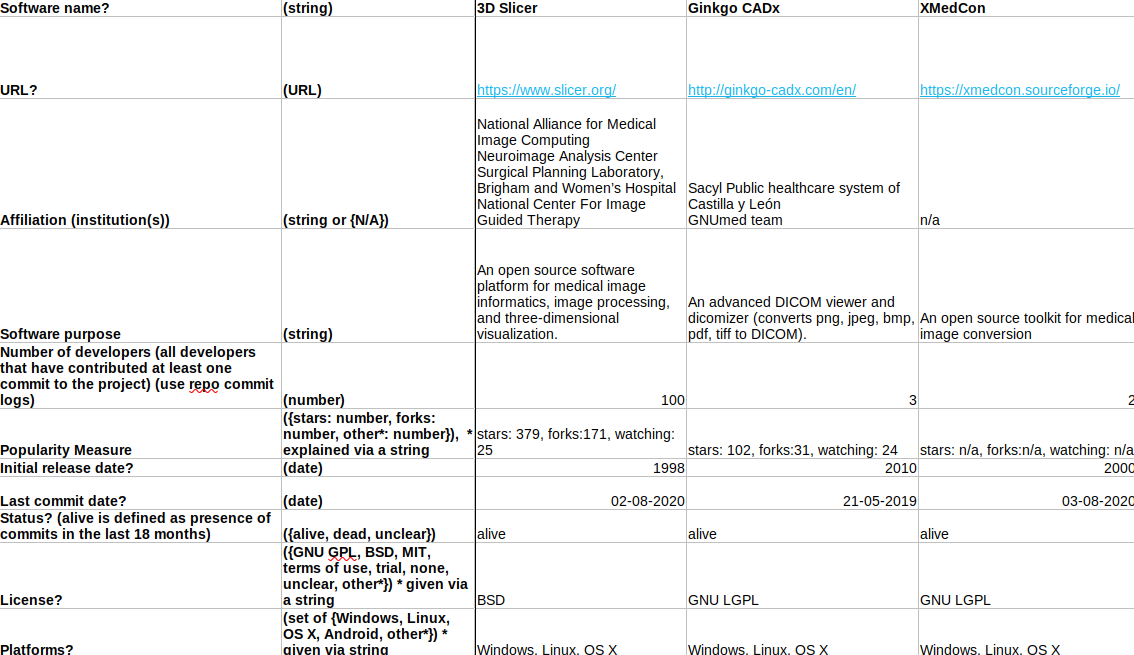
\includegraphics[scale=0.42]{figures/template.png}
\caption{Grading template example}
\label{fg_grading_template_example}
\end{figure}

We use the first section of the template to collect general information, such as the name, purpose, platform, programming language, publications about the software, the first release and the most recent change date, website, source code repository of the product, etc. Information in this section helps us understand the projects better and may be helpful for further analysis, but it does not directly affect the grading scores.

We designed the following nine sections in the template for the nine software qualities mentioned in Section \ref{sec_software_quality}. For each quality, we ask several questions and the typical answers are among the collection of ``yes'', ``no'', ``n/a'', ``unclear'', a number, a string, a date, a set of strings, etc. Each quality needs an overall score between 1 and 10 based on all the previous questions. For some qualities, we perform surface measurements, which allow us to measure all packages with reasonable efforts. The surface measurements reveal some traits of a underlying quality, but may not fully represent it.

\begin{itemize}
\item \textbf{Installability} We check the existence and quality of installation instructions. The user experience is also an important factor, such as the ease to follow the instructions, number of steps, automation tools, and the prerequisite steps for the installation. If any problem interrupts the process of installation or uninstallation, we give a lower score to this quality. We also record the Operating System (OS) for the installation test and whether we can verify the installation.

\item \textbf{Correctness \& Verifiability} For \textit{correctness}, we check the projects to identify the techniques to ensure this quality, such as literate programming, automated testing, symbolic execution, model checking, unit tests, etc. We also examine whether the projects use continuous integration and continuous delivery (CI/CD). For \textit{verifiability}, we go through the documents of the projects to check the requirements specifications, theory manuals, and getting started tutorials. If a getting started tutorial exists and provides expected results, we follow it and check if the outputs match.

\item \textbf{Surface Reliability} We check whether the software breaks during the installation and the operations following a getting started tutorials, whether there are descriptive error messages, and if we can recover the process after an error. We use the software to load damaged images during the assessment to \textit{surface robustness}, and lower its score for \textit{surface reliability} if a software product ``break" in this process.

\item \textbf{Surface Robustness} We check how the software handles unexpected/unanticipated input. For example, we prepare broken image files for MI software packages with the function to load image files. We use a text file (.txt) with a modified extension name (.dcm) as an unexpected/unanticipated input. We load a few correct input files to ensure the function is working correctly before testing with the unexpected/unanticipated ones.

\item \textbf{Surface Usability} We examine the documentation of the projects, and we consider software with a getting started tutorial and a user manual easier to use. Meanwhile, we check if users have any channels to get support. We also record our impressions and user experiences when testing the software. Easy-to-use graphical user interfaces give us a better experience, which leads to better scores.

\item \textbf{Maintainability} We search the projects' documents and identify the process of contributing and reviewing code. We believe that the artifacts of a project - including source code, documents, building scripts, etc. - can significantly affect its  \textit{maintainability}. Thus we check each project for its artifacts, such as API documentation, bug tracker, release notes, test cases, build files, version control, etc. We also check the tools supporting issue tracking and version control, the percentages of closed issues, and the proportion of comment lines in code.

\item \textbf{Reusability} We count the total number of code files for each project. Projects with a large number of components provide more choices to reuse. Furthermore, well-modularized code, which tends to have smaller parts in separated files, is typically easier to reuse. Thus, we consider the projects with more code files and less code lines per file to be more reusable. We use a command-line tool \textit{scc} to count the number of  text-based files and LOC for all projects. We also decide that the projects with API documentation can deliver better \textit{Reusability}.

\item \textbf{Surface Understandability} We randomly examine 10 code files. We check the code’s style within each file, such as whether the identifiers, parameters, indentation, and formatting are consistent, whether the constants (other than 0 and 1) are hardcoded, and whether the developers modularized the code. We also check the descriptive information for the code, such as documents mentioning the coding standard, the comments in the code, and the descriptions or links for algorithms in the code. 

\item \textbf{Visibility/Transparency} To measure this quality, we check the existing documents to find out whether the software development process and current status of a project are visible and transparent. We examine the development process, current status, development environment, and release notes for each project. If any information is missing or poorly conveyed, the \textit{visibility/transparency} will be lower.
\end{itemize}

For some qualities, the empirical measurements also affect the score. We use tools to extract information from the source code repositories. For projects held on GitHub, we manually collect additional metrics, such as the stars of the GitHub repository, and the numbers of open and closed pull requests. Section \ref{sec_empirical_measurements} presents more details about the empirical measurements.

\subsection{Empirical Measurements}
\label{sec_empirical_measurements}

We use two command-line tools for the empirical measurements. One is \textit{GitStats} that generates statistics for git repositories and displays outputs in the form of web pages \cite{Gieniusz2019}; the other one is Sloc Cloc and Code (as known as \textit{scc}) \cite{Boyter2021}, aiming to count the lines of code, comments, etc.

Both tools measure the number of text-based files in a git repository and lines of text in these files. Based on our experience, most text-based files in a repository contain programming source code, and developers use them to compile and build software products. A minority of these files are instructions and other documents. So we roughly regard the lines of text in text-based files as lines of programming code. The two tools usually generate similar but not identical results. From our understanding, this minor difference is due to the different techniques to detect if a file is text-based or binary.

Additionally, we manually collect information for projects held on GitHub, such as the numbers of stars, forks, people watching this repository, open pull requests, closed pull requests, and the number of months a repository has been on GitHub. A git repository can have a creation date much earlier than the first day on GitHub. For example, the developers created the git repository of \textit{3D Slicer} in 2002, but did not upload a copy of it to GitHub until 2020. We get the creation date of the GitHub copy by using API \textit{https://api.github.com/repos/{:owner}/{:repository}} (e.g., \hyperlink{https://api.github.com/repos/slicer/slicer}{https://api.github.com/repos/slicer/slicer}). In the response, the value of ``created\_at" is what we want. The number of months a repository has been on GitHub helps us understand the average change of metrics over time, e.g., the average new stars per month. 

These empirical measurements help us from two aspects. Firstly, they help us with getting a project overview faster and more accurately. For example, the number of commits over the last 12 months shows how active this project has been, and the number of stars and forks may reveal its popularity. Secondly, the results may affect our decisions regarding the grading scores for some software qualities. For example, if the percentage of comment lines is low, we double-check the \textit{understandability} of the code; if the ratio of open versus closed pull requests is high, we pay more attention to the \textit{maintainability}.

\subsection{Technical Details}
\label{sec_technical_details}
To test the software on a ``clean'' system, we create a new virtual machine (VM) for each software and only install the necessary dependencies before measuring. We make all 30 VMs on the same computer, one at a time, and destroy them after measuring.

We spend about two hours grading each package, unless we find technical issues and need more time to resolve them. In most of the situation, we finish all the measurements for one software on the same day.

\section{Interview Methods}
\label{sec_interview_methods}

This section introduces our interview questions (Section \ref{sec_interview_questions}), method of selecting interviewees (Section \ref{sec_interviewee_selection}), and interview process (Section \ref{sec_interview_process}).

\subsection{Interview Questions}
\label{sec_interview_questions}
We designed a list of 20 questions to guide our interviews, which can be found in Section \ref{ch_interview} and Appendix \ref{ap_interview}.

Some questions are about the background of the software, the development teams, the interviewees, and how they organize the projects. We also ask about their understandings of the users. Some questions focus on the current and past difficulties, and the solutions the team has found or will try. We also discuss the importance and current situations of documentation. A few questions are about specific software qualities, such as \textit{maintainability}, \textit{understandability}, \textit{usability}, and \textit{reproducibility}.

The interviews are semi-structured based on the question list; we ask follow-up questions when necessary. Based on our experience, the interviewees usually bring up some exciting ideas that we did not expect, and it is worth expanding on these topics.

\subsection{Interviewee Selection}
\label{sec_interviewee_selection}
For a software list with a length of roughly 30, we aim to interview about ten development teams. Interviewing multiple individuals from each team gives us more comprehensive information, but a single engineer well-knowing the project is also sufficient.

Ideally, we select projects after the grading measurements and prefer the ones with higher overall scores. However, if we do not find enough participants, we reach all teams on the list. As mentioned in Section  \ref{sec_apply_to_mi_interviews}, when we applied this process to the MI domain, we eventually contacted all teams.

We try to find the contacts of the teams on the projects' websites, such as the official web pages, repositories, publications, and bio pages of the teams' institutions. Then, we send at most two emails to one contact asking for its participation before receiving any replies. We operate the invitation according to our ethics approval, such as the one in Appendix \ref{ap_ethics}. For example, we ask for participants' consent before interviewing them, recording the conversation, or including it in our report.

\subsection{Interview Process}
\label{sec_interview_process}
Before contacting any interviewee candidate, we need to receive ethics clearance from the McMaster University Research Ethics Board. Since the members of the development teams are usually around the world, we organize these interviews as virtual meetings online with \hyperlink{https://zoom.us/}{Zoom}. After receiving consent from the interviewees, we also record and transcribe our discussions.

\section{Applying the Method to MI}
\label{sec_applying_method}
This section shows an overview of applying our method to the MI domain.

\subsection{Domain Selection}
Based on the principles in Section \ref{sec_domain_selection}, we selected the MI domain and the sub-group of software with the Visualization function shown in Figure \ref{fig_mi_functions}. We also included Dr. Michael Noseworthy, a professor of Electrical and Computer Engineering at McMaster University, Co-Director of the McMaster School of Biomedical Engineering, and Director of Medical Imaging Physics and Engineering at St. Joseph’s Healthcare, and some of his students as the MI domain experts in our team.

\subsection{Software Product Selection}
\label{sec_mi_software_selection}
By using the method in Section \ref{sec_identify_software_candidates}, we identified 48 MI software projects as the candidates from publications \cite{Bjorn2017} \cite{Bruhschwein2019} \cite{Haak2015}, online articles related to the domain \cite{Emms2019} \cite{Hasan2020} \cite{Mu2019}, forum discussions related to the domain \cite{Samala2014}, etc. Appendix \ref{ap_list_before_filtering} shows all 48 software packages.

Guided by the method in Section \ref{sec_filter_software_list}, we filtered the list with a process as follows:

\begin{enumerate}
\item Among them, there were eight that we could not find their source code, such as \textit{MicroDicom}, \textit{Aliza}, and \textit{jivex}. These packages are likely to be freeware defined in Section \ref{sec_freeware} and not OSS. So following guidelines in Section \ref{sec_filter_software_list} we removed them from the list.

\item Next, we focused on the MI software providing Visualization functions, as described in Section \ref{sec_scope}. Seven of the software on the list were Tool Kits or libraries for other software to use as dependencies, but not for end-users to view medical images, such as \textit{VTK}, \textit{ITK}, and \textit{dcm4che}; another three were PACS. We also eliminated these from the list.

\item Finally, we removed \textit{Open Dicom Viewer} from the list because it had not received any updates for a long time (since 2011). After that, only \textit{MatrixUser} and \textit{AMIDE} were considered as ``dead". However, both of them had much more recent updates (after 2017) than \textit{Open Dicom Viewer}.
\end{enumerate}

We still preferred projects using git and GitHub and being updated recently, but did not apply this filter since packages were already below 30. Even without this filter, 27 out of the 29 software packages on the filtered list used git, and 24 chose GitHub.

Following the process in Section \ref{sec_vet_software_list}, our domain experts provided a list of top software that contains 12 software products (Table \ref{tab_top_software_experts}). We compared two lists and found six common ones.

\begin{table}[H]
\centering
\begin{tabular}{ll}
\hline
Software & On both lists \\ \hline
3D Slicer & X \\
Horos & X \\
ImageJ & X \\
Fiji & X \\
AFNI &  \\
FSL &  \\
Freesurfer &  \\
Mricron & X \\
Mango & X \\
Tarquin &  \\
Diffusion Toolkit &  \\
MRItrix &  \\ \hline
\end{tabular}
\caption{\label{tab_top_software_experts}Top software by the MI domain experts}
\end{table}

We included \textit{Mango} in the initial list, but removed it because it was not OSS. However, we kept \textit{Papaya}, a the web version of \textit{Mango}. Instead of \textit{MRIcron}, we chose \textit{MRIcroGL}, because \textit{MRIcron} development had moved to
\textit{MRIcroGL} \cite{Rorden2021b}.

Six software packages on the domain experts' list were not on our filtered list. We believed their primary function was Analysis mentioned in Section \ref{sec_scope}. Thus, we did not include them in our final list.

After vetting our filtered list, the domain experts believed it was reasonable and did not identify any problem. Thus, as shown in Appendix \ref{ap_list_before_filtering}, eventually, we had 29 software products on the final list. 

\subsection{Grading Software}
\label{sec_applying_method_grading}
Then we followed the steps in Section \ref{sec_grading_software} to measure and grade the software. 27 out of the 29 packages are compatible with two or three different OS such as Windows, macOS, and Linux, and 5 of them are browser-based, making them platform-independent. However, in the interest of time, we only performed the measurements for each project by installing it on one of the platforms, most likely Windows.

\subsection{Interviews}
\label{sec_apply_to_mi_interviews}
We received ethics clearance from the McMaster University Research Ethics Board (Appendix \ref{ap_ethics}). Going through the interview process in Section \ref{sec_interview_methods}, we contacted all of the 29 teams. Members from eight teams responded and agreed to participate. As a result, we interviewed nine developers and architects from the eight teams.

\chapter{Measurement Results}
\label{ch_results}

This section shows the summary of the measurement results. The detailed data can be found in the repository \hyperlink{https://github.com/smiths/AIMSS}{https://github.com/smiths/AIMSS}.

Table \ref{tab_final_list} shows the 29 software packages that we measured. We tried to find the initial release dates (Rlsd) in the documents, such as the introduction and release notes. We did not find this date for two projects and marked them with ``?". We used the date of the latest change to each code repository to decide the latest update. We found out funding information (Fnd) for eight projects, and we are not sure about the rest.

We counted the number of contributors (NOC) and lines of code (LOC). we considered anyone who made at least one accepted commit to the source code as a contributor. Thus, it does not mean that any development team has are 100 long-term members. Many of these projects received change requests and code from the community, such as pull requests and git commits on GitHub.

Table \ref{tab_final_list} also shows the supported OS for each software package, and 25 of them could work on all three Windows (W), macOS (M), and Linux (L) systems. However, there was a significant difference in the philosophy to achieve cross-platform compatibility. Most of them were native software products, but five were naturally platform-independent web applications.

\begin{table}[H]
\begin{tabular}{llllllllll}
\hline
\multirow{2}{*}{Software} & \multirow{2}{*}{Rlsd} & \multirow{2}{*}{Updated} & \multirow{2}{*}{Fnd} & \multirow{2}{*}{NOC} & \multirow{2}{*}{LOC} & \multicolumn{3}{c}{OS} & \multirow{2}{*}{W} \\ \cline{7-9}
 &  &  &  &  &  & W & M & L &  \\ \hline
3D Slicer \cite{Kikinis2014} & 1998 & 2020-08 & X & 100 & 501451 & X & X & X &  \\
Ginkgo CADx \cite{Wollny2020} & 2010 & 2019-05 &  & 3 & 257144 & X & X & X &  \\
XMedCon \cite{Nolf2003} & 2000 & 2020-08 &  & 2 & 96767 & X & X & X &  \\
Weasis \cite{Roduit2021} & 2010 & 2020-08 &  & 8 & 123272 & X & X & X &  \\
MRIcroGL \cite{Rorden2021} & 2015 & 2020-08 &  & 2 & 8493 & X & X & X &  \\
SMILI \cite{Chandra2018} & 2014 & 2020-06 &  & 9 & 62626 & X & X & X &  \\
ImageJ \cite{Rueden2017} & 1997 & 2020-08 & X & 18 & 9681 & X & X & X &  \\
Fiji \cite{Schindelin2012} & 2011 & 2020-08 & X & 55 & 10833 & X & X & X &  \\
DicomBrowser \cite{Archie2012} & 2012 & 2020-08 &  & 3 & 5505 & X & X & X &  \\
3DimViewer \cite{TESCAN2020} & ? & 2020-03 & X & 3 & 178065 & X & X &  &  \\
Horos \cite{horosproject2020} & ? & 2020-04 &  & 21 & 561617 &  & X &  &  \\
OsiriX Lite \cite{PixmeoSARL2019} & 2004 & 2019-11 &  & 9 & 544304 &  & X &  &  \\
dwv \cite{Martelli2021} & 2012 & 2020-09 &  & 22 & 47815 & X & X & X & X \\
Drishti \cite{Limaye2012} & 2012 & 2020-08 &  & 1 & 268168 & X & X & X &  \\
\begin{tabular}[c]{@{}l@{}}BioImage Suite\\ Web \cite{Papademetris2005}\end{tabular} & 2018 & 2020-10 & X & 13 & 139699 & X & X & X & X \\
OHIF Viewer \cite{Ziegler2020} & 2015 & 2020-10 &  & 76 & 63951 & X & X & X & X \\
Slice:Drop \cite{Haehn2013} & 2012 & 2020-04 &  & 3 & 19020 & X & X & X & X \\
GATE \cite{Jan2004} & 2011 & 2020-10 &  & 45 & 207122 &  & X & X &  \\
ITK-SNAP \cite{Yushkevich2006} & 2006 & 2020-06 & X & 13 & 88530 & X & X & X &  \\
ParaView \cite{Ahrens2005} & 2002 & 2020-10 & X & 100 & 886326 & X & X & X & X \\
MatrixUser \cite{Liu2016} & 2013 & 2018-07 &  & 1 & 23121 & X & X & X &  \\
\end{tabular}
\end{table}

\begin{table}[H]
\begin{tabular}{llllllllll}
\hline
\multirow{2}{*}{Software} & \multirow{2}{*}{Rlsd} & \multirow{2}{*}{Updated} & \multirow{2}{*}{Fnd} & \multirow{2}{*}{NOC} & \multirow{2}{*}{LOC} & \multicolumn{3}{c}{OS} & \multirow{2}{*}{W} \\ \cline{7-9}
 &  &  &  &  &  & W & M & L &  \\ \hline
DICOM Viewer \cite{Afsar2021} & 2018 & 2020-04 & X & 5 & 30761 & X & X & X &  \\
INVESALIUS 3 \cite{Amorim2015} & 2009 & 2020-09 &  & 10 & 48605 & X & X & X &  \\
medInria \cite{Fillard2012} & 2009 & 2020-11 &  & 21 & 148924 & X & X & X &  \\
dicompyler \cite{Panchal2010} & 2009 & 2020-01 &  & 2 & 15941 & X & X &  &  \\
MicroView \cite{ParallaxInnovations2020} & 2015 & 2020-08 &  & 2 & 27470 & X & X & X &  \\
Papaya \cite{UTHSCSA2019} & 2012 & 2019-05 &  & 9 & 71831 & X & X & X &  \\
AMIDE \cite{Loening2017} & 2006 & 2017-01 &  & 4 & 102827 & X & X & X &  \\
Gwyddion \cite{Nevcas2012} & 2004 & 2020-11 &  & 38 & 643427 & X & X & X &  \\ \hline
\end{tabular}
\caption{\label{tab_final_list}Final software list}
\end{table}

Most of the projects used more than one programming language, including a primary language that the developers used the most. Figure \ref{fig_language} shows the primary languages versus the number of projects using them.

\begin{figure}[H]
\centering
\begin{tikzpicture}
\centering
\begin{axis}
[
ybar,
height=8cm,
width=12cm,
ylabel={Number of projects},
xlabel={\ Primary language},
symbolic x coords={C++, JavaScript, Java, C, Python, Pascal, Matlab},
xtick=data,
nodes near coords,
nodes near coords align={vertical},
]
\addplot[black,fill=blue!55!black] coordinates {(C++,11) (JavaScript,6) (Java,4) (C,3) (Python,3) (Pascal,1) (Matlab,1) };
\end{axis}  
\end{tikzpicture}
\caption{\label{fig_language}Primary languages versus number of projects using them}
\end{figure}

We failed installing \textit{DICOM Viewer}, so we could not test \textit{surface reliability} and \textit{surface robustness} for it. We kept this software on our list because the other seven qualities do not rely on a successful installation. Besides, it used a unique dependency, and we wanted to keep the diversity.

\section{Installability}
\label{sec_result_installability}

Figure \ref{fg_installability_scores} lists the scores of \textit{installability}.

\begin{figure}[H]
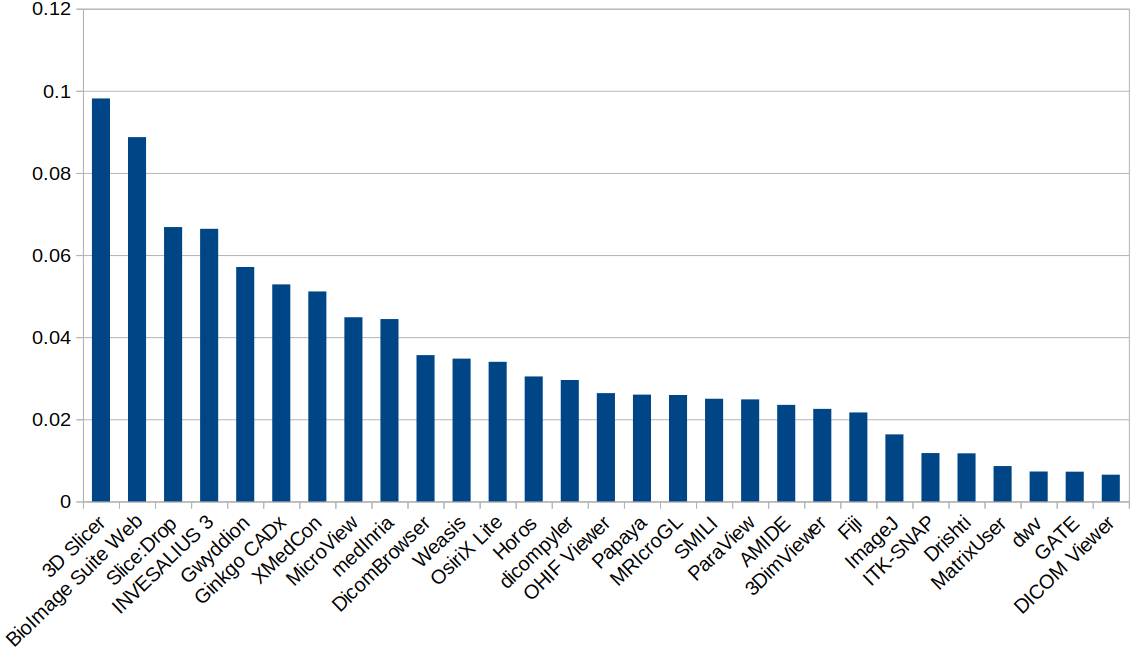
\includegraphics[scale=0.38]{figures/installability_scores.png}
\caption{AHP installability scores}
\label{fg_installability_scores}
\end{figure}

We found installation instructions for 16 projects. Among the ones without such an instruction, \textit{BioImage Suite Web} and \textit{Slice:Drop} were web applications and provided online versions to use, thus they needed no installation. Installing 10 of the projects needed extra dependencies. Five of them are the web applications in Table \ref{tab_final_list}, and depended on a browser; \textit{dwv}, \textit{OHIF Viewer}, and \textit{GATE} needed extra dependencies to build; \textit{ImageJ} and	\textit{Fiji} needed an unzip tool; \textit{MatrixUser} was based on Matlab; \textit{DICOM Viewer} needed to work on Nextcloud platform.

\textit{3D Slicer} has the highest score because it had easy-to-follow installation instructions, and the installation processes were automated, fast, and frustration-free, with all dependencies automatically added. There were also no errors during the installation and uninstallation steps. Many other software packages also had installation instructions and automated installers, and we had no trouble installing them, such as \textit{INVESALIUS 3}, \textit{Gwyddion}, \textit{XMedCon}, and \textit{MicroView}. We gave them various scores based on the understandability of the instructions, installation steps, and user experience. Since \textit{BioImage Suite Web} and \textit{Slice:Drop} needed no installation, we gave them higher scores due to the significant convenience. \textit{BioImage Suite Web} also provided an option to download cache to local for offline usage, which was easy to apply.

\textit{dwv}, \textit{GATE}, and \textit{DICOM Viewer} showed severe problems. We could not install them due to some issues that we could not solve. We spent a reasonable amount of time on these problems, then considered them major obstacles for normal users if we still did not figure out any solutions. We suspect that only a part of the users faced the same problems, and given a lot of time, we might be able to find solutions. However, the difficulties greatly impacted the installation experiences, and we graded these software packages with lower scores. For example, \textit{dwv} and \textit{GATE} had the option to build from the source code, and we failed the building processes following the instructions. Although we could not locally build them, we could use a deployed online version for \textit{dwv}, and a VM version for \textit{GATE}. With those, we finished all the measurements for them. Furthermore, \textit{DICOM Viewer} depended on a cloud platform, and we could not successfully install the dependency.

\textit{MatrixUser} has a lower score because it depended on Matlab. We considered installing Matlab takes many more steps and time, and some users may not have a license to use Matlab.

\section{Correctness \& Verifiability}
The scores of \textit{correctness \& verifiability} are shown in Figure \ref{fg_correctness_erifiability_scores}. Generally speaking, the packages with higher scores adopted more techniques to improve \textit{correctness}, and had better documents for us to verify it.

\begin{figure}[H]
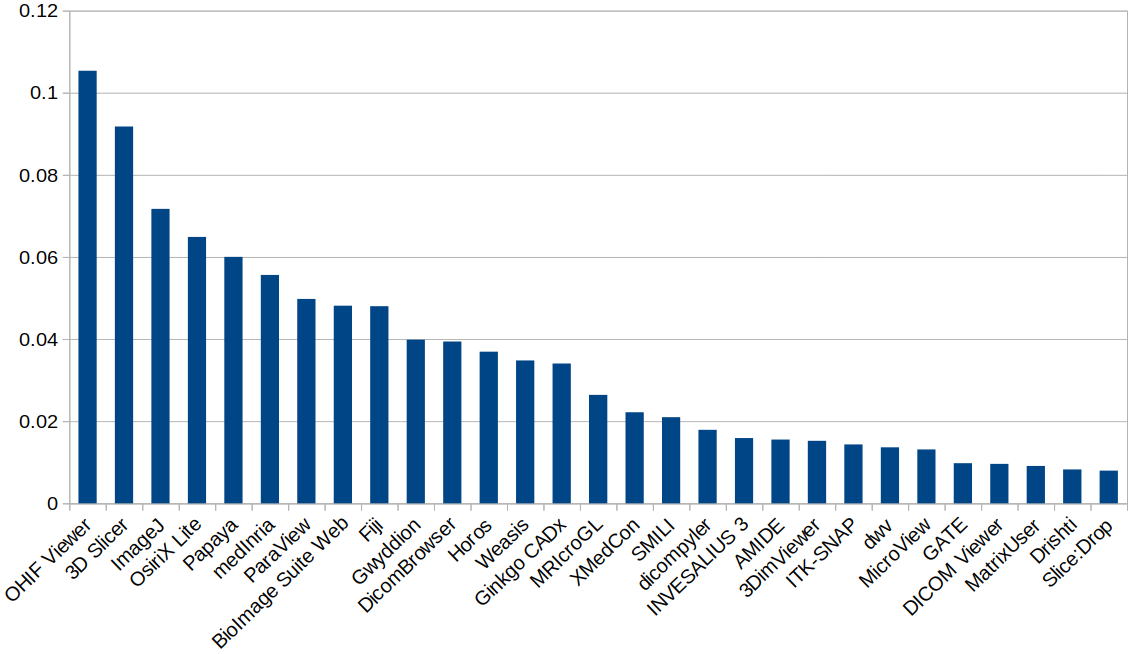
\includegraphics[scale=0.38]{figures/correctness_verifiability_scores.png}
\caption{AHP correctness \& verifiability scores}
\label{fg_correctness_erifiability_scores}
\end{figure}

After examining the source code, we could not find any evidence of unit testing in more than half of the projects. Unit testing benefits most parts of the software's life cycle, such as designing, coding, debugging, and optimization \cite{Hamill2004}. It can reveal the bugs at an earlier stage of the development process, and the absence of unit testing may cause worse \textit{correctness \& verifiability}.

We could not find requirements specifications for most projects. The only document we found is a road map of \textit{3D Slicer}, which contained design requirements for the following changes. However, it did not record the conditions for previous versions. We also could not identify the theory manuals for all of the projects. It seems that even for some projects with well-organized documents, requirements specifications and theory manuals were still missing.

We identified five projects using CI/CD tools, which are \textit{3D Slicer}, \textit{ImageJ
}, \textit{Fiji}, \textit{dwv}, and \textit{OHIF Viewer}.

\section{Surface Reliability}
As described in Section \ref{sec_result_installability}, we could not build \textit{dwv} and \textit{GATE}. However, since there was an online or VM version of them, successful deployment is possible. So the failure of installation did not affect their scores in \textit{surface reliability}. Figure \ref{fg_reliability_scores} shows the AHP results.

\begin{figure}[H]
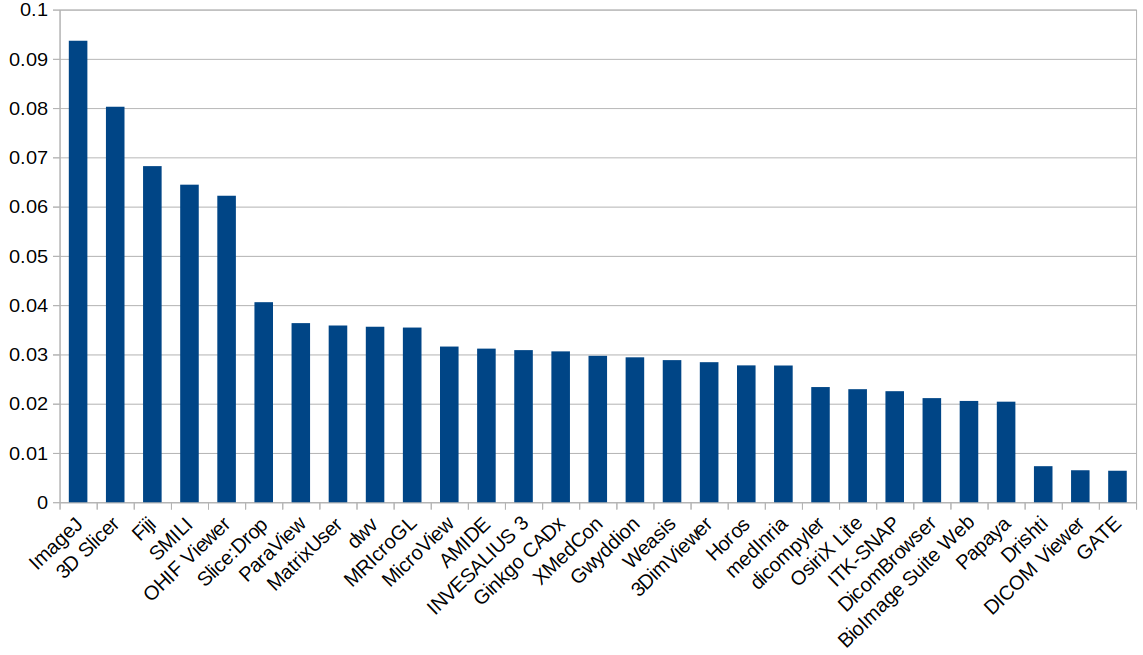
\includegraphics[scale=0.38]{figures/reliability_scores.png}
\caption{AHP surface reliability scores}
\label{fg_reliability_scores}
\end{figure}

When applying basic operations with the software packages, we found out that \textit{Drishti} crashed during loading damaged image files, and \textit{GATE} could not open macro files and lost response several times.

\section{Surface Robustness}
Figure \ref{fg_robustness_scores} presents the scores for \textit{surface robustness}.

\begin{figure}[H]
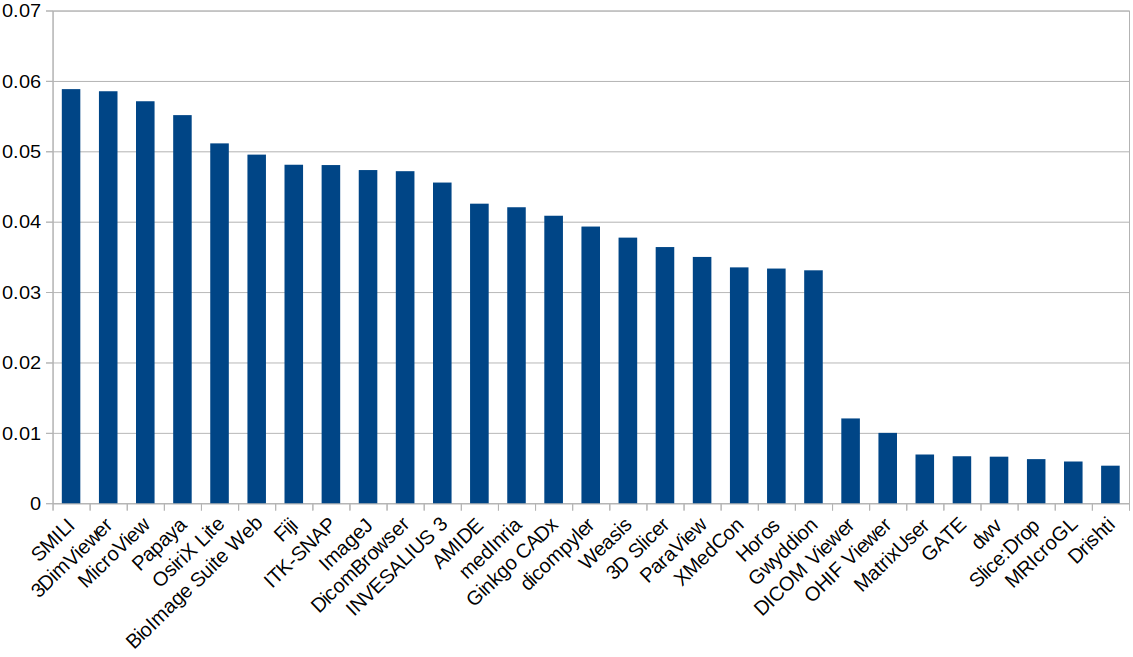
\includegraphics[scale=0.38]{figures/robustness_scores.png}
\caption{AHP surface robustness scores}
\label{fg_robustness_scores}
\end{figure}

The packages with higher scores elegantly handled the unexpected/unanticipated inputs, normally showing a clear error message. We might underestimate the score of \textit{OHIF Viewer} since we needed further customization to load data, and the test was not complete. \textit{MatrixUser}, \textit{dwv}, \textit{Slice:Drop}, and \textit{MRIcroGL} ignored the incorrect format of the input files, and displayed blank or meaningless images. \textit{Drishti} successfully detected the unexpected/unanticipated inputs, but the software crashed as a result. For unknown reasons, \textit{GATE} failed to load both correct and incorrect inputs.

\section{Surface Usability}
Figure \ref{fg_usability_scores} lists the AHP scores for \textit{surface usability}.

\begin{figure}[H]
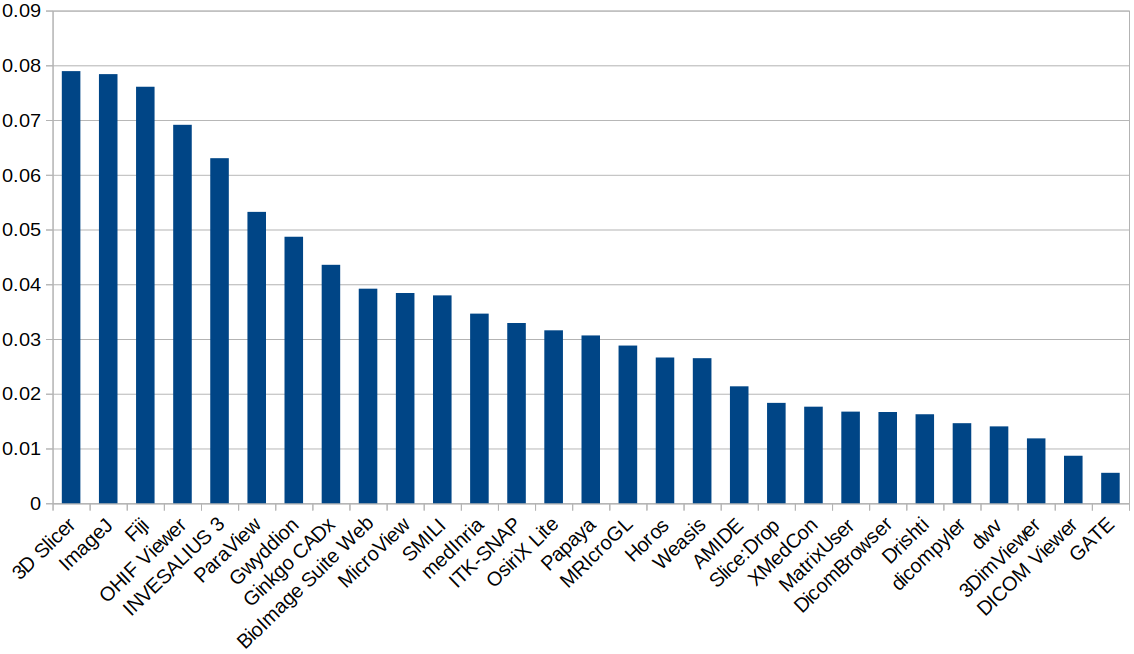
\includegraphics[scale=0.38]{figures/usability_scores.png}
\caption{AHP surface usability scores}
\label{fg_usability_scores}
\end{figure}

We found a getting started tutorial for only 11 projects but a user manual for 22 projects. \textit{MRIcroGL} was the only one with expected user characteristics documented.

The ones with higher scores usually provided both comprehensive document guidance and a good user experience. \textit{INVESALIUS 3} set an excellent example of a detailed and precise user manual. \textit{GATE} also provided a large number of documents, but we think that they conveyed the ideas poorly, as we had trouble understanding and using them.
 
Table \ref{tab_user_support_model} shows the user support models by the number of projects using them. Maybe not every team intended to use GitHub issues to answer users' questions, but many users use them to seek help.

\begin{table}[H]
\centering
\begin{tabular}{ll}
\hline
\multicolumn{1}{c}{User support model} & Number of projects \\ \hline
GitHub issue & 24 \\
GitLab issue, SourceForge discussions & 2 \\
FAQ & 12 \\
Forum & 10 \\
E-mail address & 9 \\
Troubleshooting & 2 \\
Contact form & 1 \\ \hline
\end{tabular}
\caption{\label{tab_user_support_model}User support models by number of projects}
\end{table}

\section{Maintainability}
Figure \ref{fg_maintainability_scores} shows the AHP results for \textit{maintainability}. 

\begin{figure}[H]
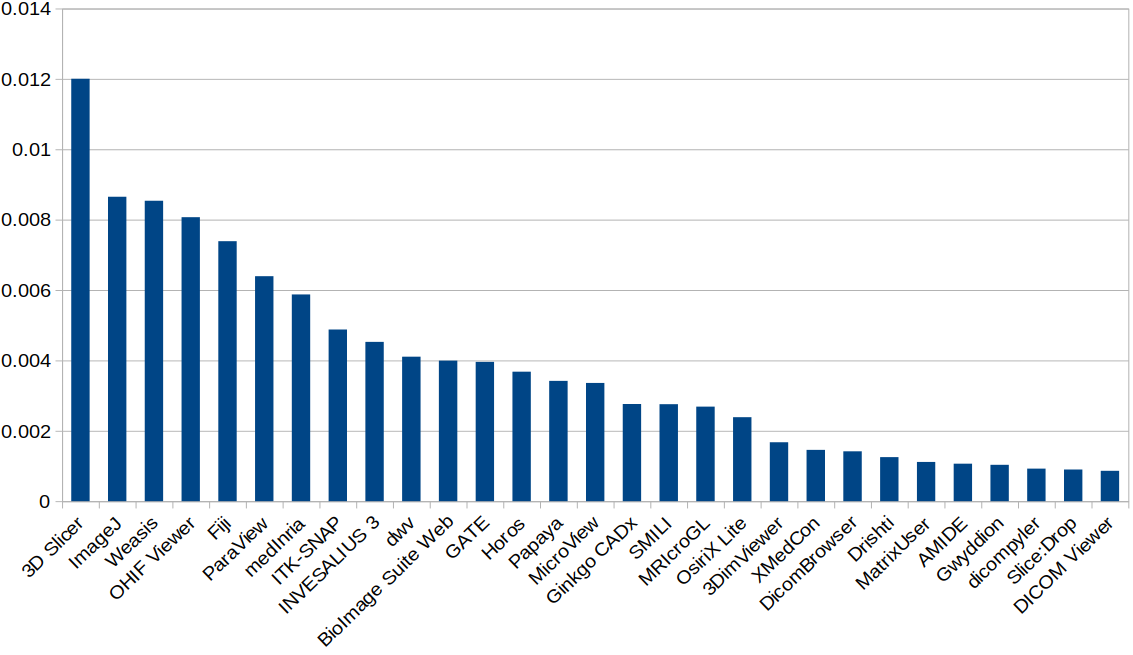
\includegraphics[scale=0.38]{figures/maintainability_scores.png}
\caption{AHP maintainability scores}
\label{fg_maintainability_scores}
\end{figure}

We marked \textit{3D Slicer} with a much higher score than others because it did very well at closing the identified issues, and more importantly, we found it to have the most comprehensive artifacts. For example, as far as we could find out, only a few of the 29 projects had a project plan, developer's manual, or API documentation, and only \textit{3D Slicer}, \textit{ImageJ}, \textit{Fiji} included all three documents. Meanwhile, \textit{3D Slicer} has a much higher percentage of closed issues (91.65\%) than \textit{ImageJ} (52.49\%) and \textit{Fiji} (63.79\%). Table \ref{tab_maintainability_docs} shows which projects had these documents.

\begin{table}[H]
\centering
\begin{tabular}{llll}
\hline
\multicolumn{1}{c}{Software} & Proj plan & Dev manual & API doc \\ \hline
3D Slicer & X & X & X \\
Weasis &  & X &  \\
SMILI &  &  & X \\
ImageJ & X & X & X \\
Fiji & X & X & X \\
dwv &  &  & X \\
BioImage Suite Web &  & X &  \\
OHIF Viewer &  & X & X \\
ParaView & X &  &  \\
INVESALIUS 3 & X &  &  \\
medInria &  & X &  \\
Gwyddion &  & X & X \\ \hline
\end{tabular}
\caption{\label{tab_maintainability_docs}Software with the maintainability documents}
\end{table}

27 of the 29 projects used git as the version control tool; \textit{AMIDE} used Mercurial; \textit{Gwyddion} used Subversion. 24 projects used GitHub for their repositories; \textit{XMedCon
}, \textit{AMIDE}, and \textit{Gwyddion} used SourceForge; \textit{DicomBrowser} and \textit{3DimViewer} used BitBucket.

\section{Reusability}
Figure 4.7 shows the AHP results for \textit{reusability}.

\begin{figure}[H]
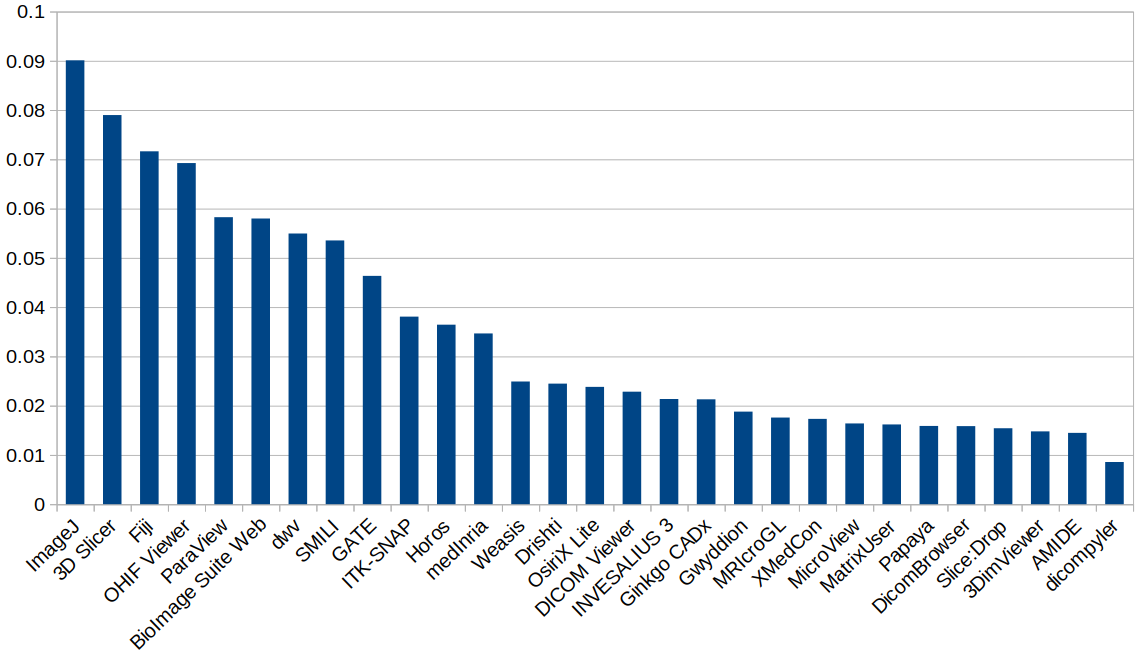
\includegraphics[scale=0.38]{figures/reusability_scores.png}
\caption{AHP reusability scores}
\label{fg_reusability_scores}
\end{figure}

As described in Section \ref{sec_grading_template}, we gave higher scores to the projects with an API document and more code files. As shown in Table \ref{tab_maintainability_docs}, seven projects had API documents. Figure \ref{fg_num_text_files} shows the number of text-based files by projects.

\begin{figure}[H]
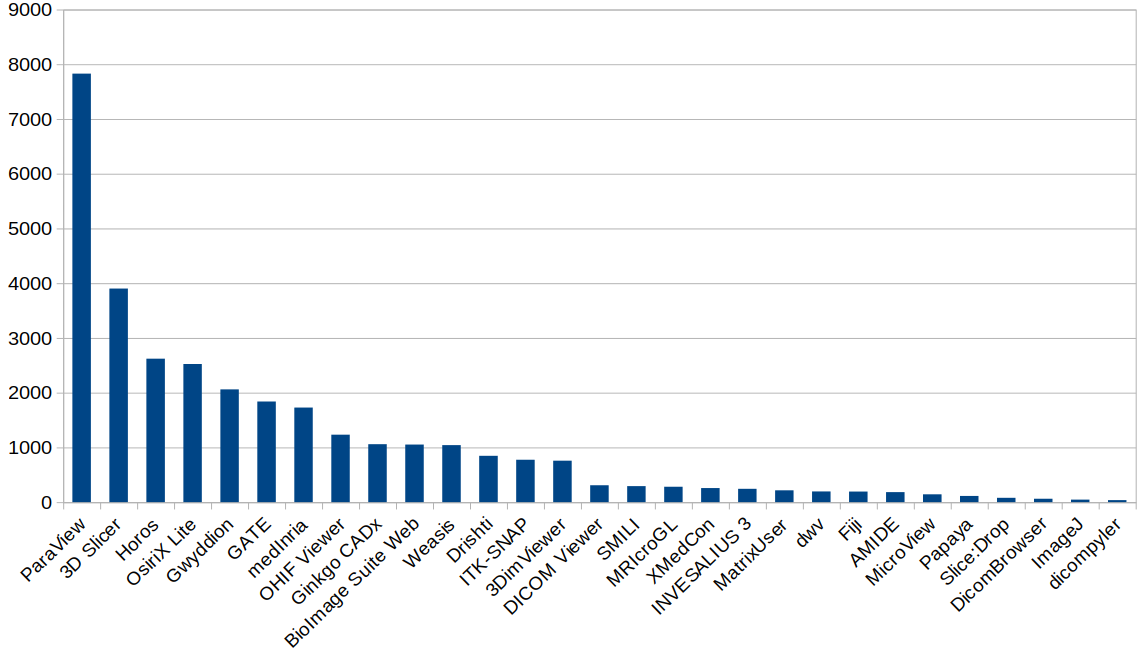
\includegraphics[scale=0.38]{figures/num_text_files.png}
\caption{Number of text-based files files by projects}
\label{fg_num_text_files}
\end{figure}

\section{Surface Understandability}
Figure \ref{fg_surface_understandability_scores} shows the scores for \textit{surface understandability}.

\begin{figure}[H]
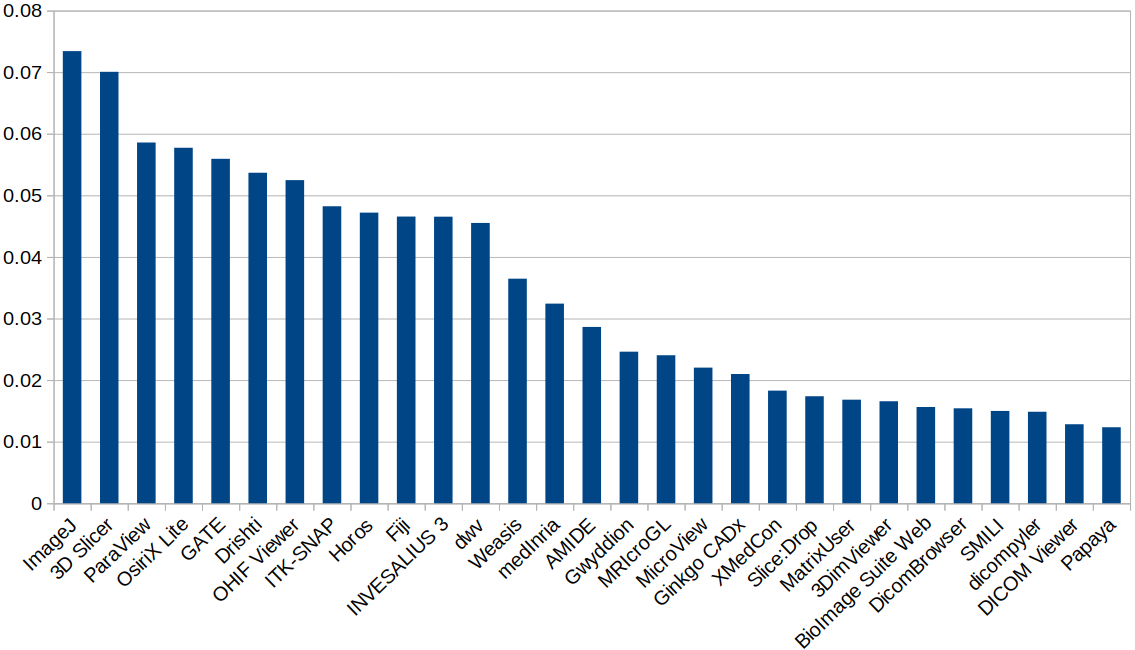
\includegraphics[scale=0.38]{figures/understandability_scores.png}
\caption{AHP surface understandability scores}
\label{fg_surface_understandability_scores}
\end{figure}

All projects had a consistent code style with parameters in the same order for all functions; the code was modularized; the comments were clear, indicating what is being done, not how. However, we only found explicit identification of a coding standard for only 3 out of the 29, which are \textit{3D Slicer}, \textit{Weasis}, and \textit{ImageJ}. We also found hard-coded constants in \textit{medInria}, \textit{dicompyler}, \textit{MicroView}, and \textit{Papaya}. We did not find any reference to the used algorithms in projects \textit{XMedCon}, \textit{DicomBrowser}, \textit{3DimViewer}, \textit{BioImage Suite Web}, \textit{Slice:Drop}, \textit{MatrixUser}, \textit{DICOM Viewer}, \textit{dicompyler}, and \textit{Papaya}. 

\section{Visibility/Transparency}
Figure \ref{fg_visibility_transparency_scores} shows the AHP scores for \textit{visibility/transparency}. Generally speaking, the teams that actively documented their development process and plans scored higher because they delivered better communication to people outside the team.

\begin{figure}[H]
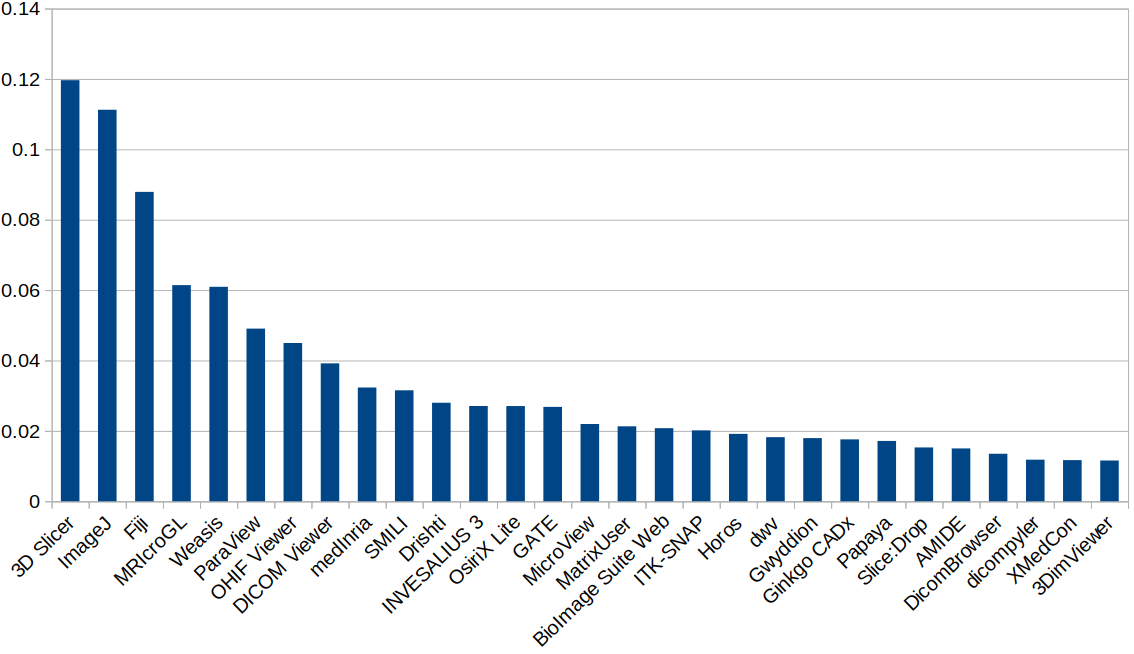
\includegraphics[scale=0.38]{figures/visibility_transparency_scores.png}
\caption{AHP visibility/transparency scores}
\label{fg_visibility_transparency_scores}
\end{figure}

Table \ref{tab_Visibility/Transparency_docs} shows the projects which had documents for the development process, project status, development environment, and release notes.

\begin{table}[]
\centering
\begin{tabular}{lllll}
\hline
Software & Dev process & Proj status & Dev env & Rls notes \\ \hline
3D Slicer & X & X & X & X \\
Weasis \cite{Roduit2021} &  &  & X & X \\
MRIcroGL \cite{Rorden2021} &  &  &  & X \\
SMILI \cite{Chandra2018} &  &  &  & X \\
ImageJ \cite{Rueden2017} & X & X & X & X \\
Fiji \cite{Schindelin2012} & X & X & X &  \\
Horos \cite{horosproject2020} &  &  &  & X \\
OsiriX Lite \cite{PixmeoSARL2019} &  &  &  & X \\
dwv \cite{Martelli2021} &  &  &  & X \\
Drishti \cite{Limaye2012} &  &  &  & X \\
\begin{tabular}[c]{@{}l@{}}BioImage Suite\\ Web\end{tabular} &  &  & X &  \\
OHIF Viewer \cite{Ziegler2020} &  &  & X & X \\
GATE \cite{Jan2004} &  &  &  & X \\
ITK-SNAP \cite{Yushkevich2006} &  &  &  & X \\
ParaView \cite{Ahrens2005} &  & X &  &  \\
MatrixUser \cite{Liu2016} &  &  &  & X \\
DICOM Viewer \cite{Afsar2021} &  &  & X & X \\
INVESALIUS 3 \cite{Amorim2015} &  &  &  & X \\
medInria \cite{Fillard2012} &  &  & X & X \\
MicroView \cite{ParallaxInnovations2020} &  &  &  & X \\
Gwyddion \cite{Nevcas2012} &  &  &  & X \\ \hline
\end{tabular}
\caption{\label{tab_Visibility/Transparency_docs}Software with the visibility/transparency documents}
\end{table}

\section{Overall Scores}

As described in Section \ref{sec_AHP}, for our AHP measurements, there are nine criteria which are the nine software qualities and 29 software packages as the alternatives. We decided to make all nine qualities equally important, so the score of each quality affects the overall scores on the same scale.

Figure \ref{fg_overall_scores} shows the overall scores of all 29 software packages in descending order. Since we produced the scores from the AHP process, the total sum of the 29 scores is precisely 1.

\begin{figure}[H]
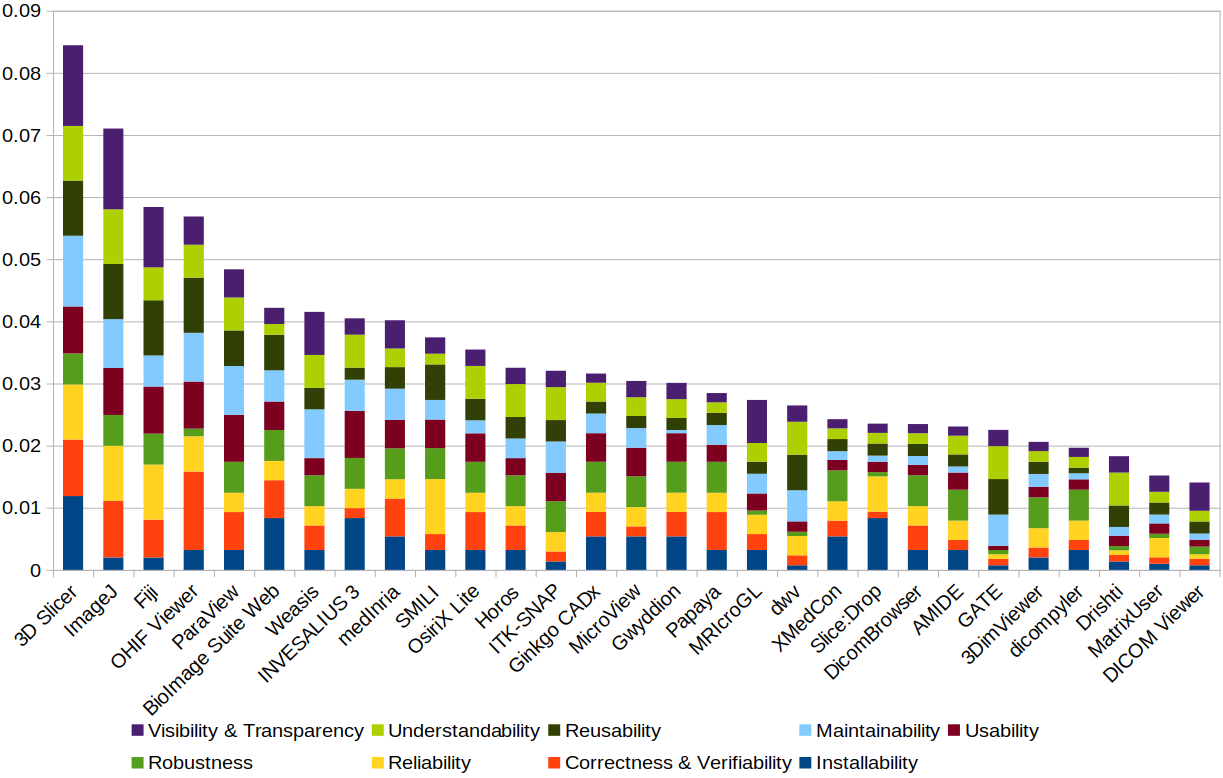
\includegraphics[scale=0.38]{figures/overall_scores.png}
\caption{Overall AHP scores for all 9 software qualities}

\label{fg_overall_scores}
\end{figure}

The top three software products \textit{3D Slicer}, \textit{ImageJ}, and \textit{OHIF Viewer} had higher scores in most criteria. \textit{3D Slicer} ranked in the top two software products for all qualities except \textit{surface robustness}; \textit{ImageJ} ranked in the top three products for \textit{correctness \& verifiability}, \textit{surface reliability}, \textit{surface usability}, \textit{maintainability}, \textit{ surface understandability}, and \textit{visibility/transparency}; \textit{OHIF Viewer} ranked in the top five products for \textit{correctness \& verifiability}, \textit{surface reliability}, \textit{surface usability}, \textit{maintainability}, and \textit{reusability}. We might underestimate its scores of qualities \textit{surface reliability} and \textit{surface robustness} for \textit{DICOM Viewer}, but equally compared it with the other software for the rest seven qualities.

\chapter{Interviews with Developers}
\label{ch_interviews}

\section{Summary of Answers}

\begin{itemize}
\item Start with one by one, with commonalities and interesting special cases.

\item Shorten and summarize later.
\end{itemize}

\section{Discussions}

Any conclusions?

\chapter{Threat to Validity}
\label{ch_validity}

\chapter{Recommendations}
\label{ch_recommendations}

\section{Recommendations to Software Qualities}

We list some of the key points that may improve each quality as follows,
\begin{itemize}
\item \textbf{Installability}
\begin{itemize}
    \item clear instructions;
    \item automated installer;
    \item including all dependencies in the installer;
    \item avoiding heavily depending on other commercial products (e.g. Matlab);
    \item considering building a web application that needs no installation.
\end{itemize}
\item \textbf{Correctness \& Verifiability}
\begin{itemize}
    \item test-driven development with unit tests, integration tests, nightly tests, etc.
    \item two stage development process with stable release \& nightly builds;
    \item CI/CD;
    \item documents of requirements specifications and theory manuals.
\end{itemize}
\item \textbf{Reliability}
\begin{itemize}
    \item test-driven development with unit tests, integration tests, nightly tests, etc.
    \item two stage development process with stable release \& nightly builds;
    \item descriptive error messages.
\end{itemize}
\item \textbf{Robustness}
\begin{itemize}
    \item designing with exceptions and make the software failures elegant;
    \item descriptive error messages.
\end{itemize}
\item \textbf{Usability}
\begin{itemize}
    \item usability tests and interviews with end users;
    \item adjusting according to users’ feedbacks;
    \item getting started tutorials;
    \item user manuals;
    \item professional UX designs;
    \item active supports to users.
\end{itemize}
\item \textbf{Maintainability}
\begin{itemize}
    \item using GitHub;
    \item modular approach;
    \item documentation for developers, such as project plan, developer’s manual, and API documentation.
\end{itemize}
\item \textbf{Reusability}
\begin{itemize}
    \item modular approach;
    \item API documentation.
\end{itemize}
\item \textbf{Understandability}
\begin{itemize}
    \item modular approach;
    \item consistent codding style;
    \item clear comments;
    \item description of used algorithms;
    \item documentation;
    \item communication between developers and users via GitHub issues, mailing lists, forums etc.
    \item graphical user interface.
\end{itemize}
\item \textbf{Visibility/Transparency}
\begin{itemize}
    \item documents for the development process, project status, development environment, and release notes.
\end{itemize}
\item \textbf{Reproducibility}
\begin{itemize}
    \item test-driven development with unit tests, integration tests, nightly tests, etc.
    \item open-source;
    \item making data and documentation available;
    \item using open-source libraries.
\end{itemize}
\end{itemize}

\chapter{Conclusions}
\label{ch_conclusions}

We analyzed the state of the practice for SC software in the MI domain. To better achieve our goals in Section \ref{ch_intro}, we proposed six research questions in Section \ref{sec_research_questions}.

Our methods in Section \ref{ch_methods} form a general process to evaluate domain-specific software, that we apply on specific SC domains. As mentioned in Section \ref{sec_applying_method}, following this process, we chose the MI domain, identified 48 SC software candidates in it, then selected 29 of them to our final list. Section \ref{ch_results} lists our measurements to nine software qualities for the 29 projects, and Section \ref{ch_interview} contains our interviews with eight of the 29 teams, discussing their development process and five software qualities.

We answered our six research questions in Section \ref{ch_answers}. In addition, Section \ref{ch_recommendations} presents our recommendations on SC software development.

\section{Key Findings}

With the measurement results in Section \ref{ch_results}, we revealed some current status of SC software development and qualities in the MI domain. We ranked the 29 software projects in nine qualities based on the grading scores. \textit{3D Slicer}, \textit{ImageJ}, and \textit{OHIF Viewer} are the top three software by their overall scores.

The interview results in Section \ref{ch_interview} show some merits, drawbacks, and pain points within the development process. The three primary categories of pain points are:
\begin{itemize}
\item the lack of fundings and time;
\item the difficulty to balance between four factors: cross-platform compatibility, convenience to development \& maintenance, performance, and security;
\item the lack of access to real-world datasets for testing.
\end{itemize}
We summarized the solutions from the developers to address these problems. We also collected the status of software testing, documentation, contribution management, and project management in the eight projects.

Our answers to the research questions (Section \ref{ch_answers}) are based on the above findings. We identified the existing artifacts, tools, principles, processes, and methodologies in the 29 projects. By comparisons in Section \ref{sec_rq_comparison}, we found out: 1) four of the top five software projects in our ranking were also among the top five ones receiving the most GitHub stars per year (Table \ref{tab_ranking_vs_GitHub}); 2) three of the top four in our ranking were among the top four provided by the domain experts (Table \ref{tab_top_software_vs_experts}).

Section \ref{ch_recommendations} presents our recommendations on improving software qualities and easing pain points during development. Some highlighted ones are:
\begin{itemize}
\item adopting test-driven development with unit tests, integration tests, and nightly tests;
\item maintaining good documentation (e.g., installation instructions, requirements specifications, theory manuals, getting started tutorials, user manuals, project plan, developer’s manual, API documentation, requirements on coding standards, development process, project status, development environment, and release notes);
\item using CI/CD;
\item using git and GitHub;
\item modular approach with the design principle proposed by Parnas \cite{ParnasEtAl2000};
\item considering newer technologies (e.g., web application and serverless solution);
\item various ways of enriching the testing datasets in Section \ref{sec_recommendations_testing_dataset}.
\end{itemize}

\section{Future Works}

With learnings from this project, we summarized recommendations for the future state of the practice assessments:
\begin{itemize}
    \item we can make the surface measurements less shallow. For example:
    \begin{itemize}
        \item \textit{surface reliability}: our current measurement relies on the processes of installation and getting started tutorials. However, not all software needs installation or has a getting started tutorial. We can design a list of operation steps, perform the same operations with each software, and record any errors.
        \item \textit{surface robustness}: we used damaged images as inputs for this measuring MI software. This process is similar to fuzz testing \cite{enwiki:1039424308}, which is one type of fault injection \cite{enwiki:1039005082}. We may adopt more fault injection methods, and identify tools and libraries to automate this process.
        \item \textit{surface usability}: we can design usability tests and test all software projects with end-users. The end-users can be volunteers and domain experts.
        \item \textit{surface understandability}: our current method does not require understanding the source code. As software engineers, perhaps we can select a small module of each project, read the source code and documentation, try to understand the logic, and score the ease of the process.
    \end{itemize}
	\item we can further automate the measurements on the grading temple in Appendix \ref{ap_grading_template}. For example, with automation scripts and a GitHub API, we may save significant time on retrieving the GitHub metrics;
	\item the grading standard can be more explicit. For example, we can explicitly define scores for each item in the grading temple.
	\item we can improve some interview questions. Some examples are:
	\begin{itemize}
	    \item in \hyperlink{q14}{Q14}, ``Do you think improving this process can tackle the current problem?" is a yes-or-no question, which is not informative enough. As mentioned in Section \ref{sec_contribution_pm}, most interviewees ignored it. We can change it to ``By improving this process, what current problems can be tackled?";
	    \item in \hyperlink{q16}{Q16}, we can ask more details about the modular approach, such as "What principles did you use to divide code into modules? Can you give an example of using the principles?";
	    \item \hyperlink{q17}{Q17} and  \hyperlink{q18}{Q18} should respectively ask \textit{understandability} to developers and \textit{usability} to end-users.
	\end{itemize}
	\item we can better organize the interview questions. Since we use audio conversion tools to transcribe the answers, we should make the transcription easier to read. For example, we can order them together for questions about the five software qualities and compose a similar structure for each.
	\item we can mark the follow-up interview questions with keywords. For example, say ``this is a follow-up question" every time asking one. Thus, we record this sentence in the transcription, and it will be much easier to distinguish the follow-up questions from the 20 designed questions.
\end{itemize}

\noindent In addition, we propose a few SC domains that are potentially suitable for future works:
\begin{itemize}
    \item Metallurgy
    \item Quantitative Finance
    \item Computational Fluid Dynamics
    \item Basic Linear Algebra
    \item Finite Elements
    \item Sparse Linear Solvers
\end{itemize}

\noindent After applying our method on various domains, we can start a meta-study to compare the state of the practice for software in different domains.


\addcontentsline{toc}{chapter}{Bibliography}
%\bibliographystyle{plain}
\bibliography{thesis}


\appendix
\chapter{Full Grading Template}
\label{ap_grading_template}

appendix here
\chapter{Summary of Measurements}
\label{ap_measurements}

appendix here
\chapter{Other Interview Answers}
\label{ap_interview}

We asked 20 interview questions to the nine interviewees from eight software projects. We discuss the answers to interview questions 5, 9, 10, 11, 12, 13, 14, and 19 in Section \ref{ch_interview}, and summarize the answers to the other questions in this section.

\noindent\textbf{Q1. Interviewees’ current position/title? degrees?}

Six of the nine interviewees revealed their position/title, such as CEO of a company, endowed chair and professor in universities, software engineers in a commercial company and a hospital.

Most of them answered their backgrounds and degrees. Table \ref{tab_q1_degrees} shows the highest academic degrees the participants have, and Table \ref{tab_q1_majors} shows what majors they studied. Many of the interviewees studied in multiple majors.

\begin{table}[H]
\centering
\begin{tabular}{ll}
\hline
Highest degree & Number of interviewees \\ \hline
PHD & 4 \\
Master & 3 \\
Bachelor & 0 \\
Unspecified academic degree & 2 \\ \hline
\end{tabular}
\caption{\label{tab_q1_degrees}Interviewees' highest academic degrees}
\end{table}

\begin{table}[H]
\centering
\begin{tabular}{ll}
\hline
Major & Number of interviewees \\ \hline
Computer Science & 4 \\
Physics & 2 \\
Biomedical Engineering & 1 \\
Neuroimaging & 1 \\
Geology (image analysis) & 1 \\
Media Arts and Sciences & 1 \\
Mechanical Engineering & 1 \\
Materials Engineering & 1 \\
Psychology & 1 \\ \hline
\end{tabular}
\caption{\label{tab_q1_majors}Interviewees' majors at university}
\end{table}

\noindent\textbf{Q2. Interviewees’ contribution to/relationship with the software?}

Table \ref{tab_q2_roles} shows the interviewees’ roles and responsibilities in the projects. One of the participants did not explicitly mention his role, but implicitly revealed that he was a primary contributor to the project.

\begin{table}[H]
\centering
\begin{tabular}{ll}
\hline
Role in the projects & Number of interviewees \\ \hline
Chief Architect & 2 \\
Lead Developer & 1 \\
Core Developer & 5 \\
Unspecified & 1 \\ \hline
\end{tabular}
\caption{\label{tab_q2_roles}Interviewees' roles in the projects}
\end{table}

\noindent\textbf{Q3. Length of time the interviewee has been involved with this software?}

Table \ref{tab_q3_years} shows the distribution of the lengths of time the interviewees had worked on the projects.

\begin{table}[H]
\centering
\begin{tabular}{ll}
\hline
Length of time in the projects & Number of interviewees \\ \hline
0-1 & 1 \\
2-5 & 0 \\
6-10 & 2 \\
11-15 & 3 \\
16-20 & 2 \\
21-25 & 1 \\ \hline
\end{tabular}
\caption{\label{tab_q3_years}Lengths of time that the interviewees worked in the projects}
\end{table}

\noindent\textbf{Q4. How large is the development group?}

The size of each group grows and shrinks over the years. Most teams mentioned that the team members join and leave. Some teams said that when there was sufficient funding, they could afford more developers.

Table \ref{tab_q4_members} shows the numbers of active members at the time of interviews. The members include people working on development and project management.

\begin{table}[H]
\centering
\begin{tabular}{ll}
\hline
Number of current members & Number of projects \\ \hline
1-3 & 5 \\
4-6 & 3 \\ \hline
\end{tabular}
\caption{\label{tab_q4_members}Numbers of current members in the projects}
\end{table}

As shown in the table, no team had a vast number of members. Some projects had more developers, such as \textit{3D Slicer}; on the other hand, some teams such as \textit{dwv} had only one primary developer, plus a maximum of two or three developers occasionally.

\textit{3D Slicer} is a special case, because it supports third-party extensions. So there have been community members developing and maintaining these extensions. Table \ref{tab_q4_members} does not include these members.

\noindent\textbf{Q6. What is the typical background of a developer?}

Not all interviewees could clearly answer this question. Many of them talked about the backgrounds of members with who they were familiar. Table \ref{tab_q6_dev_backgrounds} shows the number of times all interviewees mentioned a background.

\begin{table}[H]
\centering
\begin{tabular}{ll}
\hline
Background of a developer & Number of interviewees with the answer \\ \hline
\begin{tabular}[c]{@{}l@{}}Computer Science, Information\\ Technology, and Software Development \end{tabular} & 6 \\
Imaging & 2 \\
Medical Imaging & 1 \\
Mathematics & 1 \\
Biomedical Engineering & 1 \\
Computer Aided Medical Procedures & 1 \\
Physician & 1 \\ \hline
\end{tabular}
\caption{\label{tab_q6_dev_backgrounds}Backgrounds of developers by the numbers of interviewees with the answers}
\end{table}

\noindent\textbf{Q7. What is your estimated number of users? How did you come up with that estimate?}

None of the interviewees knew the exact number of users. Some of them provided estimations based on different facts. However, we do not think these numbers are comparable to each other.

\begin{table}[H]
\centering
\begin{tabular}{lll}
\hline
Software & Rough estimation & Considered facts \\ \hline
3D Slicer & 100,000 & \begin{tabular}[c]{@{}l@{}} Search results on Google Scholar;\\ number of new posts per year on slicer.org; \\ number of downloads. \end{tabular} \\
INVESALIUS 3 & 75,000 & Number of random IDs created by new installation.\\
dwv & No estimation & About 20 companies integrated \textit{dwv} in their products. \\
BioImage Suite Web & 100 active users & \begin{tabular}[c]{@{}l@{}}  The  interviewee only counted the users from \\ several Universities who were active users. \end{tabular} \\
ITK-SNAP & 10,000 plus & Number of downloads. \\
MRIcroGL & No estimation & \begin{tabular}[c]{@{}l@{}}  It is the top 1 downloaded software on this NITRC list \\ \hyperlink{https://www.nitrc.org/top/toplist.php?type=downloads}{https://www.nitrc.org/top/toplist.php?type=downloads} \end{tabular} \\
Weasis & \begin{tabular}[c]{@{}l@{}}  10,000 user used \\ it as least once \end{tabular} & Number of profiles. \\
OHIF & About 5000 & \begin{tabular}[c]{@{}l@{}}   Some platforms integrated \textit{OHIF}, and it was hard \\ to know the number of end users. \end{tabular} \\ \hline
\end{tabular}
\caption{\label{tab_q7_num_users}Rough Estimations for the Number of Users}
\end{table}

Table \ref{tab_q7_num_users} shows the estimations and how the interviewees made them. It is clear that some estimated only the active users, and some counted users who had used only once. So we do not compare these numbers.

\noindent\textbf{Q8. What is the typical background of a user?}

All interviewees provided several different user backgrounds, and all of them mentioned medical researchers or medical professionals. Table \ref{tab_q8_user_backgrounds} shows the number of times all interviewees mentioned a background.

\begin{table}[H]
\centering
\begin{tabular}{ll}
\hline
Background of a user & Number of interviewees with the answer \\ \hline
Medical Researchers & 6 \\
Doctors/Health care professionals/Surgeons & 5 \\
Student Researchers & 4 \\
Patients & 3 \\
Paleontologist & 1 \\
Biomechanical Engineers & 1 \\
Imaging Researchers & 1 \\
Mechanical Engineers & 1 \\ \hline
\end{tabular}
\caption{\label{tab_q8_user_backgrounds}Backgrounds of users by the numbers of interviewees with the answers}
\end{table}

\noindent\textbf{Q15. Was it hard to ensure the correctness of the software? If there were any obstacles, what methods have been considered or practiced to improve the situation? If practiced, did it work?}

Table \ref{tab_q15_threats_correctness} shows the threats to \textit{correctness} by the numbers of interviewees with the answers.

\begin{table}[H]
\centering
\begin{tabular}{ll}
\hline
Threat to correctness & Number of interviewees with the answer \\ \hline
\begin{tabular}[c]{@{}l@{}}Clinical systems produce data in various formats \\ (e.g. DICOM), which have complicated standards.\\ The software needs to handle the complexity.\end{tabular} & 2 \\
\begin{tabular}[c]{@{}l@{}}Different types of MI machines can create data \\ in slightly different ways, adding more complexity\\ for the software to handle.\end{tabular} & 2 \\
\begin{tabular}[c]{@{}l@{}}Besides viewing, the software has additional \\ functions, which lead to extra complexity.\end{tabular} & 1 \\
There is lack of real word image data for testing. & 1 \\
\begin{tabular}[c]{@{}l@{}}The team cannot use private data for debugging,\\ even when the data cause problems.\end{tabular} & 1 \\
\begin{tabular}[c]{@{}l@{}}The software uses huge datasets for testing, so \\ the tests are expensive and time-consuming.\end{tabular} & 1 \\
It is hard to well manage releases. & 1 \\
The project has no unit tests. & 1 \\
The project has no dedicated quality assurance team. & 1 \\ \hline
\end{tabular}
\caption{\label{tab_q15_threats_correctness}Threats to correctness by the numbers of interviewees with the answers}
\end{table}

Table \ref{tab_q15_strategies_correctness} shows the strategies to ensure \textit{correctness} by the numbers of interviewees with the answers. The interviewees from the \textit{3D Slicer} and \textit{ITK-SNAP} teams thought that the self-tests and automated tests were beneficial and could significantly save time. The interviewee from the \textit{Weasis} team kept collecting medical images for more than ten years. These images have caused problems with the software. So he had samples to test specific problems.

\begin{table}[H]
\centering
\begin{tabular}{ll}
\hline
Strategy to ensure correctness & Number of interviewees with the answer \\ \hline
\begin{tabular}[c]{@{}l@{}}Test-driven development / component tests /\\ integration tests / smoke tests / regression tests.\end{tabular} & 4 \\
Self tests / automated tests. & 3 \\
\begin{tabular}[c]{@{}l@{}}Two stage development process / stable release \&\\ nightly builds.\end{tabular} & 3 \\
CI/CD. & 1 \\
\begin{tabular}[c]{@{}l@{}}Using deidentified copies of medical images for\\ debugging.\end{tabular} & 1 \\
\begin{tabular}[c]{@{}l@{}}Sending the beta versions of software to medical\\ workers who can access the data and do the tests.\end{tabular} & 1 \\
\begin{tabular}[c]{@{}l@{}}Collecting and maintaining a dataset of\\ problematic images.\end{tabular} & 1 \\ \hline
\end{tabular}
\caption{\label{tab_q15_strategies_correctness}Strategies to ensure correctness by the numbers of interviewees with the answers}
\end{table}

\noindent\textbf{Q16. When designing the software, did you consider the ease of future changes? For example, will it be hard to change the system’s structure, modules, or code blocks? What measures have been taken to ensure the ease of future changes and maintains?}

Table \ref{tab_q16_strategies_maintainability} shows the strategies to ensure \textit{maintainability} by the numbers of interviewees with the answers. The modular approach is the most talked-about solution to improve \textit{maintainability}. The \textit{3D Slicer} team used a well-defined structure for the software, which they named as ``event-driven MVC pattern''. Moreover, \textit{3D Slicer} discovers and loads necessary modules at runtime, according to the configuration and installed extensions. The \textit{BioImage Suite Web} team had designed and re-designed their software multiple times in the last 10+
years. They found that their modular approach effectively supported the maintainability \cite{Joshi2011}. 

\begin{table}[H]
\centering
\begin{tabular}{ll}
\hline
Strategy to ensure maintainability & Number of interviewees with the answer \\ \hline
\begin{tabular}[c]{@{}l@{}}Modular approach / thinking the software\\ as reusable Lego bricks / maintain \\ repetitive functions as libraries.\end{tabular} & 5 \\
Supporting third-party extensions. & 1 \\
Easy-to-understand architecture. & 1 \\
Dedicated architect. & 1 \\
Starting from simple solutions. & 1 \\
Documentation. & 1 \\ \hline
\end{tabular}
\caption{\label{tab_q16_strategies_maintainability}Strategies to ensure maintainability by the numbers of interviewees with the answers}
\end{table}

\noindent\textbf{Q17. Provide instances where users have misunderstood the software. What, if any, actions were taken to address understandability issues?}

Table \ref{tab_q17_threats_understandability} shows the threats to \textit{understandability} by the numbers of interviewees with the answers. It separates \textit{understandability} issues to users and developers by the horizontal dash line.

\begin{table}[H]
\centering
\begin{tabular}{ll}
\hline
Threat to understandability & Number of interviewees with the answer \\ \hline
\begin{tabular}[c]{@{}l@{}}Not all users understand how to use some\\ features of the software.\end{tabular} & 2 \\
\begin{tabular}[c]{@{}l@{}}The team has no dedicated user experience\\ (UX) designer.\end{tabular} & 1 \\
\begin{tabular}[c]{@{}l@{}}The software does not make some important\\ indicators noticeable (e.g. a progress bar).\end{tabular} & 1 \\
\begin{tabular}[c]{@{}l@{}}Not all users understand the purpose of the\\ software.\end{tabular} & 1 \\
\begin{tabular}[c]{@{}l@{}}Not all users know if the software includes\\ certain features.\end{tabular} & 1 \\
\begin{tabular}[c]{@{}l@{}}Not all users understand how to use the\\ command line tool.\end{tabular} & 1 \\
\begin{tabular}[c]{@{}l@{}}Not all users understand that the software is \\a web application.\end{tabular} & 1 \\\hdashline
\begin{tabular}[c]{@{}l@{}}Not all developers understand how to deploy\\ the software.\end{tabular} & 1 \\
\begin{tabular}[c]{@{}l@{}}The architecture is difficult for new\\ developers to understand.\end{tabular} & 1 \\ \hline
\end{tabular}
\caption{\label{tab_q17_threats_understandability}Threats to understandability by the numbers of interviewees with the answers}
\end{table}

Table \ref{tab_q17_strategies_understandability} shows the strategies to ensure \textit{understandability} by the numbers of interviewees with the answers.

\begin{table}[H]
\centering
\begin{tabular}{ll}
\hline
Strategy to ensure understandability & Number of interviewees with the answer \\ \hline
\begin{tabular}[c]{@{}l@{}}Documentation / user manual /\\ user mailing list / forum.\end{tabular} & 4 \\
Graphical user interface. & 2 \\
Testing every release with active users. & 1 \\
\begin{tabular}[c]{@{}l@{}}Making simple things simple and complicated\\ things possible.\end{tabular} & 1 \\
Icons with more clear visual expressions. & 1 \\
Designing the software to be intuitive. & 1 \\
Having a UX designer with the right experience. & 1 \\
Dialog windows for important notifications. & 1 \\
\begin{tabular}[c]{@{}l@{}}Providing an example if the users need to build\\ the software by themselves.\end{tabular} & 1 \\ \hline
\end{tabular}
\caption{\label{tab_q17_strategies_understandability}Strategies to ensure understandability by the numbers of interviewees with the answers}
\end{table}

\noindent\textbf{Q18. What, if any, actions were taken to address usability issues?}

Table \ref{tab_q18_strategies_usability } shows the strategies to ensure \textit{usability} by the numbers of interviewees with the answers.

\begin{table}[H]
\centering
\begin{tabular}{ll}
\hline
Strategy to ensure usability & Number of interviewees with the answer \\ \hline
Usability tests and interviews with end users. & 3 \\
Adjusting according to users' feedbacks. & 3 \\
\begin{tabular}[c]{@{}l@{}}Straightforward and intuitively designed interface /\\ professional UX designer.\end{tabular} & 2 \\
\begin{tabular}[c]{@{}l@{}}Providing step-by-step processes, and showing\\ the step numbers.\end{tabular} & 1 \\
\begin{tabular}[c]{@{}l@{}}Making the basic functions easy to use without\\ reading the documentation.\end{tabular} & 1 \\
Focusing on limited number of functions. & 1 \\
Making the software more streamlined. & 1 \\
Downsampling images to consume less memory. & 1 \\
\begin{tabular}[c]{@{}l@{}}An option to load only part of the data to boost\\ performance.\end{tabular} & 1 \\ \hline
\end{tabular}
\caption{\label{tab_q18_strategies_usability }Strategies to ensure usability by the numbers of interviewees with the answers}
\end{table}

\noindent\textbf{Q20. Do you have any concern that your computational results won’t be reproducible in the future? Have you taken any steps to ensure reproducibility?}

Table \ref{tab_q20_threats_reproducibility} shows the threats to \textit{reproducibility} by the numbers of interviewees with the answers.

\begin{table}[H]
\centering
\begin{tabular}{ll}
\hline
Threat to reproducibility & Number of interviewees with the answer \\ \hline
\begin{tabular}[c]{@{}l@{}}If the software is closed-source, the reproducibility\\is hard to achieve.\end{tabular} & 1 \\
The project has no user interaction tests. & 1 \\
The project has no unit tests. & 1 \\
\begin{tabular}[c]{@{}l@{}}Using different versions of some common libraries\\may cause problems.\end{tabular} & 1 \\
CPU variability can leads to non-reproducibility. & 1 \\
\begin{tabular}[c]{@{}l@{}}When reverse-engineering how manufacturers create\\medical images, the team may misinterpret it.\end{tabular} & 1 \\ \hline
\end{tabular}
\caption{\label{tab_q20_threats_reproducibility}Threats to reproducibility by the numbers of interviewees with the answers}
\end{table}

Table \ref{tab_q20_strategies_ reproducibility } shows the strategies to ensure \textit{ reproducibility} by the numbers of interviewees with the answers. The interviewee from the \textit{3D Slicer} team provided various suggestions. One interviewee from another team suggested that they used \textit{3D Slicer} as the benchmark to test their \textit{reproducibility}.

\begin{table}[H]
\centering
\begin{tabular}{ll}
\hline
Strategy to ensure reproducibility & Number of interviewees with the answer \\ \hline
Regression tests / unit tests / having good tests. & 6 \\
\begin{tabular}[c]{@{}l@{}}Making code, data, and documentation available / making\\ the software open-source / using open-source libraries.\end{tabular} & 5 \\
Running same tests on all platforms. & 1 \\
\begin{tabular}[c]{@{}l@{}}A dockerized version of the software,  insulating it from\\ the operating system environment.\end{tabular} & 1 \\
Using standard libraries. & 1 \\
Monitoring the upgrades of the libraries. & 1 \\
Clearly documenting the versions. & 1 \\
\begin{tabular}[c]{@{}l@{}}Bringing along the exact versions of all the dependencies\\ with the software.\end{tabular} & 1 \\
Providing checksums of the data. & 1 \\
\begin{tabular}[c]{@{}l@{}}Benchmark the software against other software with\\ similar purposes.\end{tabular} & 1 \\ \hline
\end{tabular}
\caption{\label{tab_q20_strategies_ reproducibility }Strategies to ensure  reproducibility by the numbers of interviewees with the answers}
\end{table}

\chapter{Ethics Approval}
\label{ap_ethics}
This project received ethics clearance from the McMaster Research Ethics Board on February 20, 2021. \newline

\noindent Project Title: AIMSS - State of the Practice \newline

\noindent MREB\#: 5219

\end{document}
